%====================================================
%	CHAPTER 4 - Control
%====================================================
\chapter{Controller Development}
\label{ch:control}
%====================================================
\section{Control Loop}
\label{sec:control.loop}
%====================================================
The control problem here is, as outlined in Ch:\ref{ch:intro}, to achieve non-zero set-point tracking (\emph{attitude and position} states) on a quadrotor by solving the problem of its inherent under-actuation. For the purposes of the subsequent controller development, the plant is described in the following typical non-linear state space form:
\begin{subequations}\label{eq:control-loop-states}
\begin{equation}
\frac{d}{dt}{\vec{\mathbf{x}}}=f(\vec{\mathbf{x}},t)+g(\vec{\mathbf{x}},\vec{\nu},t)
\end{equation}
\vspace{-12pt}
\begin{equation}
\vec{y} = c(\vec{\mathbf{x}},t)+d(\vec{\mathbf{x}},\vec{\nu},t)
\end{equation}
\end{subequations}
Where the plant's dynamics are governed by state progression $f(\vec{\mathbf{x}},t)$ and the plant's input response $g(\vec{\mathbf{x}},\vec{\nu},t)$ for a given control input $\vec{\nu}$. The latter could take the affine form; $g(\mathbf{x},t)\vec{\nu}$. Set-point tracking aims for the output to track the plant's state; namely $\vec{y} = c(\vec{\mathbf{x}},t)=\vec{\mathbf{x}}$. As such, the control problem is to design a stabilizing control law $h$ for some error state $\mathbf{x}_e$:
\begin{equation}
\vec{\nu}_d=h(\mathbf{x}_e,t)=h(\mathbf{x}_b,\dot{\mathbf{x}}_b,\mathbf{x}_d,\dot{\mathbf{x}}_d,t)
\end{equation}
Such that the controlled plant is asymptotically stabilizing or that $\lim_{t\rightarrow\infty}\mathbf{x}_e=0$. Trajectory stability conditions are further defined next in Sec:\ref{sec:control.stability}. Note that it is possible to combine attitude and position states into a single common trajectory state such that:
\\
\vspace{-5pt}
\begin{equation}
\vec{\mathbf{x}}=\begin{bmatrix}\vec{\mathcal{E}}&Q_b\end{bmatrix}^T
\end{equation}
The body's trajectory is then fully described by $\vec{\mathbf{x}}(t)$. Separate control laws are developed for attitude and position tracking and hence those states are not combined in the context of this control project. However for the purposes of describing the control plant, a single major loop is considered.
\par
Because of the plant's overactuatedness the control loop is split into two blocks; first a higher level \emph{set-point tracking} controller designs a virtual control input $\vec{\nu}_d$. That being net forces $\vec{F}_d$ and torques $\vec{\tau}_d$ to act on the body. A lower level \emph{allocator} then solves for explicit actuator positions from $\vec{\nu}_d$ to physically actuate that \emph{virtual} control input. The actuator set then implements a commanded control input $\vec{\nu}_c$ through its effectiveness function (Eq:\ref{eq:dynamic-plant-inputs})
\begin{equation}
\vec{\nu}_c=B(\vec{\mathbf{x}},u,t)
\end{equation}
The allocator solves for actuator values $u\in\mathbb{U}$ such that $\vec{\nu}_c\rightarrow\vec{\nu}_d$. That allocation function, $B^\dagger$, can be \emph{roughly} referred to as the effectiveness inverse:
\begin{equation}
\underset{\in\mathbb{U}}{u}=B^{\dagger}(\vec{\mathbf{x}},\vec{\nu}_d,t)
\end{equation}
This chapter derives higher level controllers for $\vec{\nu}_d=h(\vec{\mathbf{x}}_e,t)$; allocation rules are discussed next in Ch:\ref{ch:allocation}. A collection of attitude and position controllers are presented here whose stability is proven with Lyapunov theorem \cite{bojelayupanov,lyapunovstabilitytheorem,noteonlyapunov}. Each controller is compared in the context of an over actuated quadrotor plant. Similarly a series of proposed allocation schemes are presented. Controller comparisons, their details and efficacy are evaluated is subsequently in Ch:\ref{ch:simulation}. 
\par
A generalized over-actuated control loop consists of a series of cascaded control blocks (Fig:\ref{fig:control-loop}). From the trajectory's error state $\vec{\mathbf{x}}_e$, a control law designs a virtual control input $\vec{\nu}_d$ which is applied to the allocation block. The allocation law $B^{\dagger}(\mathbf{x},\vec{\nu}_d,t)$ solves for physical actuator positions $u\in\mathbb{U}$. Actuator positions command a physical input $\vec{\nu}_c=B(\mathbf{x},u,t)$ which is an input to the state's dynamics, Eq:\ref{eq:control-loop-states}. Finally the output tracking state is estimated with some filter $\hat{\mathbf{x}}=A(\mathbf{x},t)$ which is used to calculate the error state (Sec:\ref{sec:simulation.state}).
\begin{figure}[htbp]
\centering
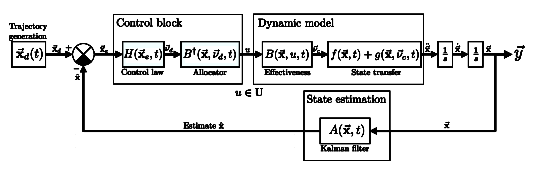
\includegraphics[width=\textwidth]{figs/control-loop}
\caption{Generalized control loop with allocation}
\vspace{-12pt}
\label{fig:control-loop}
\end{figure}
\par
Fig:\ref{fig:control-loop} is a generalized illustration of the control loop's structure; the plant's dynamics from Eq:\ref{eq:quaternion-states} include state derivative feedback. Moreover aspects of the state transfer function includes multi-body non-linearities dependent on actuator positions and rates as detailed in Sec:\ref{sec:dynamics.nonlinearities}. That generalized case is now refined in the context of an over-actuated quadcopter.
%====================================================
\section{Control Plant Inputs}
\label{sec:control.inputs}
%====================================================
Control inputs for the differential state equations, from Eq:\ref{eq:quaternion-states}, have mostly been described with net forces and torques; $\vec{F}_\mu(u)$ and $\vec{\tau}_\mu(u)$. The relationship (\emph{effectiveness function}) between each propeller's rotational speed and servo positions with the produced thrust vector is calculated from Eq:\ref{eq:quaternion-inputs}.
\begin{subequations}\label{eq:control-input}
\begin{equation}
\vec{\nu}_c\triangleq\begin{bmatrix}
\vec{F}_\mu(u) & \vec{\tau}_\mu(u)
\end{bmatrix}^T=B(\vec{\mathbf{x}},u,t)~~~~\in\mathbb{R}^6,~u\in\mathbb{U}
\end{equation}
\vspace{-10pt}
\begin{equation}
\vec{F}_\mu(u)=\sum_{i=1}^4 Q_{M_i}^*(\lambda_i,\alpha_i)\otimes T(\Omega_i)\otimes Q_{M_i}(\lambda_i,\alpha_i)~~~~\in\mathcal{F}^b
\end{equation}
\vspace{-4pt}
\begin{equation}
\vec{\tau}_\mu(u)=\sum_{i=1}^4 \vec{L}_i\times\big(Q_{M_i}^*(\lambda_i,\alpha_i)\otimes T(\Omega_i)\otimes Q_{M_i}(\lambda_i,\alpha_i)\big)~~~~\in\mathcal{F}^b
\end{equation}
\end{subequations}
As mentioned previously, a higher level controller designs desired net plant inputs $\vec{\nu}_d=\begin{bmatrix}\vec{F}_d&\vec{\tau}_d\end{bmatrix}^T$ whilst a lower level allocator commands physical inputs $u=B^{\dagger}(\vec{\mathbf{x}},\vec{\nu}_d,t)$. This allows for independent comparison of proposed control and allocation laws. However, typical allocation rules like pseudo-inversion require an affine relationship between plant and control inputs (Sec:\ref{subsubsec:intro.lit.control.allocation}). The relationship in Eq:\ref{eq:control-input} is not reducible to a single multiplicative relationship with the actuator matrix $u\in\mathbb{U}$. So the effectiveness function needs an extra layer of abstraction to incorporate a multiplicative relationship. Rather than calculating explicit actuator positions directly from $\vec{\nu}_d$; a set of four 3-D thrust vectors $\vec{T}_{1\rightarrow 4}$ for each motor module are first calculated.
\begin{subequations}\label{eq:4.7}
\begin{equation}
\vec{\nu}_c=\begin{bmatrix}
\vec{F}_\mu(u)\\
\vec{\tau}_\mu(u)
\end{bmatrix}
= 
\begin{bmatrix}
1 & 1 & 1 & 1\\
[\vec{L}_1]_\times & [\vec{L}_2]_\times & [\vec{L}_3]_\times & [\vec{L}_4]_\times
\end{bmatrix}
\begin{bmatrix}
\vec{T}_1&
\vec{T}_2&
\vec{T}_3&
\vec{T}_4
\end{bmatrix}^T
\end{equation}
\begin{equation}
\rightarrow\vec{\nu}_f=B'(\vec{\mathbf{x}},t)\begin{bmatrix}
\vec{T}_1&
\vec{T}_2&
\vec{T}_3&
\vec{T}_4
\end{bmatrix}^T
\end{equation}
\end{subequations}
Where $[\vec{L}_i]_\times$ is the cross product vector of the $i^{th}$ torque arm. Explicit actuator positions for each module, $[\Omega_i,\lambda_i,\alpha_i]^T$, can then be solved from those thrust vectors $\vec{T}_i$ for $i\in[1:4]$ with some trigonometry, "unwinding" transformations applied in Eq:\ref{eq:control-input}. That trigonometric inversion is detailed later in Sec:\ref{sec:allocation.slack} but is described as the function $R^\dagger$:
\begin{equation}\label{eq:4.8}
[\Omega_i,~\lambda_i,~\alpha_i]^T=R^\dagger(\mathbf{x},\vec{T}_i,t)~~~~\text{for}~i\in[1:4]
\end{equation}
The generalized control loop illustrated in Fig:\ref{fig:control-loop} is extended to include the abstracted allocation blocks of Eq:\ref{eq:4.7} and Eq:\ref{eq:4.8}, shown in Fig:\ref{fig:control-block}. The net control block still solves for the same actuator matrix $u\in\mathbb{U}$. The entire loop accommodates for comparison of various $B^\dagger(\mathbf{x},\vec{\nu}_d,t)$ allocation rules without having to redesign the remainder of the loop's structure.
\begin{figure}[htbp]
\vspace{-8pt}
\centering
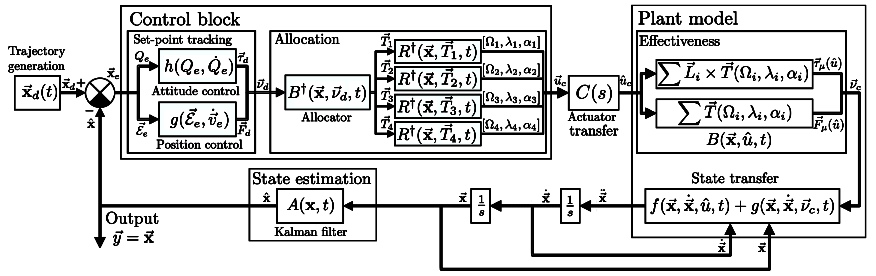
\includegraphics[width=0.95\textwidth]{figs/control-block}
\caption{Extended control loop with over-actuation}
\label{fig:control-block}
\vspace{-16pt}
\end{figure}
\par
In summary; each controller designs a net force and torque to act on the body. Allocation rules decompose that virtual input into four separate 3-D thrust vectors, or 12 directional components. The force components are an abstracted allocation layer in place of explicit actuator positions, which are subsequently solved for\ldots
\begin{equation}
B^{\dagger}(\mathbf{x},\vec{\nu}_d,t)=\big[ T_{1x},~T_{1y},~T_{1z},~\ldots~T_{4x},~T_{4y},~T_{4z}\big]^T
\end{equation}
Each control law is co-dependent on an accompanying allocation algorithm. Traditional control loops (under-actuated or well matched) typically have a unity allocation rule and as such require no consideration so they're mostly disregarded. Separate control laws for attitude ad position control are presented in Section:\ref{sec:control.attitude} and \ref{sec:control.position} respectively. Thereafter a series of allocation rules are proposed in Ch:\ref{ch:allocation}. Although presented independently, the controller and allocation laws are mutually inclusive. The stability of each controller is proven objectively but explicit controller coefficients are optimized in the subsequent Ch:\ref{ch:simulation}, in Sec:\ref{sec:simulation.tuning}.
\newpage
%====================================================
\section{Stability}
\label{sec:control.stability}
%====================================================
Before undertaking the control plant derivations, it is worth outlining definitions of what the control objectives are. The research question aims to achieve non-zero set-point tracking of state's trajectory. A control loop then aims to \emph{stabilize} the dynamics described previously in Sec:\ref{sec:dynamics.model} whilst tracking particular trajectories for attitude and position, $\mathbf{x}_d(t)=[\vec{\mathcal{E}}_d(t)~Q_d(t)]^T$. 
\par
The entire system's control loop was previously detailed in Sec:\ref{sec:control.loop}. Stability in the context of trajectory tracking must be defined. Generalized trajectory stability definitions are not uncommon in the context of energy based control design, or Lyapunov theorem (Sec:\ref{sec:control.lyapunov}). Stability definitions pertinent to Lyapunov's stability theorem are briefly presented here; the following is adapted from \cite{bojelayupanov,lyapunovstabilitytheorem}. In general for some autonomous trajectory $\vec{\mathbf{x}}(t)$, an equilibrium point $\vec{\mathbf{x}}(t_0)$ is said to be stable (\textbf{S}) if and only if (\emph{iff}) the following is true:
\begin{subequations}\label{eq:basic-stability}
\begin{equation}
\forall\varepsilon>0,~\exists~\delta_0(t_0,\varepsilon):~\norm{\vec{\mathbf{x}}(t_0)}<\delta_0(t_0,\varepsilon)
\end{equation}
\vspace{-20pt}
\begin{equation}
\Rightarrow\norm{\vec{\mathbf{x}}(t)}<\varepsilon,~~\forall t\geq t_0
\end{equation}
\end{subequations}
The implication of which is that if, for some initial condition $\vec{\mathbf{x}}(t_0)$ whose magnitude is bound by the manifold $\delta_0(t_0,\varepsilon)$, the entire subsequent trajectory of $\vec{\mathbf{x}}(t)$ is bound from above by some other manifold $\varepsilon$. Basic stability is illustrated in Fig:\ref{fig:basic-stability} for a 2-D trajectory.
\begin{figure}[hbtp]
\vspace{-6pt}
\centering
\begin{subfigure}{0.49\textwidth}
\centering
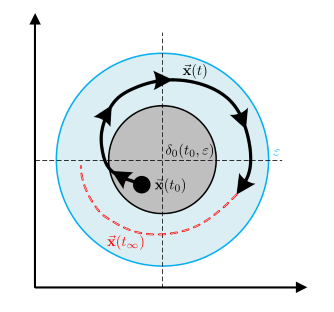
\includegraphics[width=\textwidth]{figs/basic-stability}
\vspace{-16pt}
\caption{Basic stability}
\label{fig:basic-stability}
\end{subfigure}
\begin{subfigure}{0.49\textwidth}
\centering
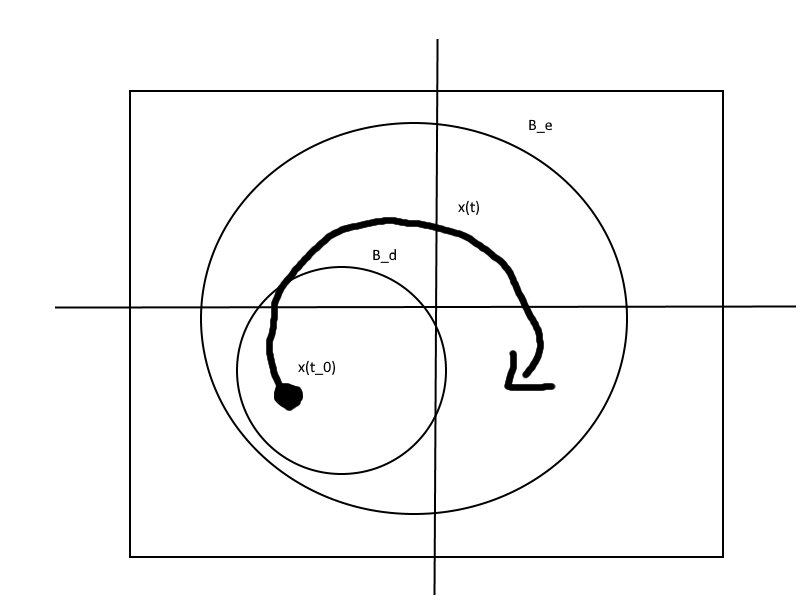
\includegraphics[width=\textwidth]{figs/uniform-stability}
\vspace{-16pt}
\caption{Uniform stability}
\label{fig:uniform-stability}
\end{subfigure}
\vspace{-8pt}
\caption{Trajectory illustrations for $\mathbf{S}$ and $\mathbf{US}$}
\vspace{-18pt}
\end{figure}
\par
An equilibrium point is further said to be uniformly stable (\textbf{US}) \emph{iff} for the time $t\in[t_0,\infty)$ the following criteria, being an extension of basic stability, is met:
\begin{subequations}\label{eq:uniform-stability}
\begin{equation}
\forall\varepsilon>0,~\exists~\delta_0(\varepsilon)>0:~\norm{\vec{\mathbf{x}}(t_1)}<\delta_0(\varepsilon),~~t_1>t_0
\end{equation}
\vspace{-18pt}
\begin{equation}
\Rightarrow\norm{\vec{\mathbf{x}}(t)}<\varepsilon,~~\forall
t\geq t_1
\end{equation}
\end{subequations}
\textbf{US} similarly bounds a trajectory from above by $\varepsilon$ if the trajectory originates from within $\delta_0(\varepsilon)$. The difference is that the principle trajectory region $\delta_0(\varepsilon)$ is independent of $t_0$ in the case of \textbf{US}. The two surfaces are effectively non-concentric; a $\mathbf{US}$ trajectory is illustrated in Fig:\ref{fig:uniform-stability}. Uniform stability is a subset of general stability, $\mathbf{US}\subset\mathbf{S}$, however the converse is not true. Furthermore \textbf{US} is a stronger assertion of stability. 
\par
Extending stability definitions to include settling; an equilibrium point is said to be asymptotically stable (\textbf{AS}) \emph{iff} conditions for \textbf{S} are met (Eq:\ref{eq:basic-stability}) and that the following holds true:
\begin{subequations}\label{eq:asymptotic-stability}
\begin{equation}
\exists~\delta_1(t_0,\varepsilon) >0:~\norm{\vec{\mathbf{x}}(t_0)}<\delta_1(t_0,\varepsilon)
\end{equation}
\vspace{-18pt}
\begin{equation}
\Rightarrow \lim_{t\rightarrow\infty}\norm{\vec{\mathbf{x}}(t)}\rightarrow 0
\end{equation}
\end{subequations}
This asserts that trajectories originating within some finer region $\delta_1(t_0,\varepsilon)$, being a subset of $\delta_0(t_0,\varepsilon)$, the trajectory tends to and \emph{asymptotically} settles at the origin. In the case of \textbf{AS} the origin is both \underline{stable} and \underline{attractive} (shown in Fig:\ref{fig:asymptotic-stability}). Asymptotic stability is typically the first requirement for any control law, being a stronger stability than both \textbf{US} and \textbf{S}\ldots
\begin{figure}[hbtp]
\centering
\begin{subfigure}{0.49\textwidth}
\centering
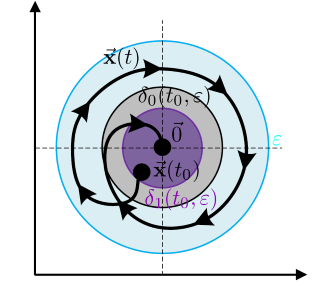
\includegraphics[width=\textwidth]{figs/asymptotic-stability}
\vspace{-8pt}
\caption{Asymptotic stability}
\label{fig:asymptotic-stability}
\end{subfigure}
\begin{subfigure}{0.49\textwidth}
\centering
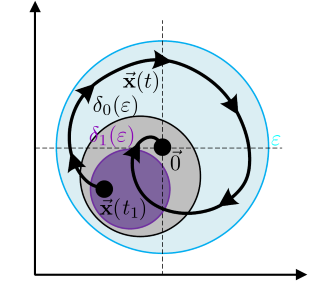
\includegraphics[width=\textwidth]{figs/uniform-asymptotic-stability}
\vspace{-8pt}
\caption{Uniform asymptotic stability}
\label{fig:uniform-asymptotic-stability}
\end{subfigure}
\vspace{-4pt}
\caption{Trajectory illustrations for $\mathbf{AS}$ and $\mathbf{UAS}$}
\vspace{-14pt}
\end{figure}
\par
Uniform asymptotic stability (\textbf{UAS}), an extension of uniform stability, occurs when the asymptotically stable bound region $\delta_1(\epsilon)$ is independent of the principle starting $t_0$. An equilibrium point is \textbf{UAS} \emph{iff} conditions for \textbf{S} are met and that:
\begin{subequations}\label{eq:uniform-asymptotic-stability}
\begin{equation}
\exists~\delta_1(\varepsilon)>0:~\norm{\vec{\mathbf{x}}(t_1)}<\delta_1(\varepsilon),~~t_1\geq t_0
\end{equation} 
\vspace{-16pt}
\begin{equation}
\Rightarrow \lim_{t\rightarrow\infty}\norm{\vec{\mathbf{x}}(t)}\rightarrow 0
\end{equation}
\end{subequations}
A uniformly asymptotic equilibrium point implies stability from a non-concentric ball of attraction; settling to the origin (illustrated in Fig:\ref{fig:uniform-asymptotic-stability}). 
\par
An equilibrium point is regarded as exponentially stable (\textbf{UES}) if conditions for \textbf{UAS} are met and that there exist $\exists~a,b,r$ that bound the settling of the trajectory such that:
\begin{equation}\label{eq:exponential-stability}
\norm{\vec{\mathbf{x}}(t,t_0,\vec{\mathbf{x}}_0)}\leq a\norm{\vec{\mathbf{x}}_0}e^{-bt},~~\forall\norm{\vec{\mathbf{x}}_0}\leq r
\end{equation}
The term $a\norm{\vec{\mathbf{x}}_0}e^{-bt}$ bounds the rate at which the trajectory settles to the origin, illustrated in Fig:\ref{fig:exponential-stability}. The initial point of the trajectory, $\vec{\mathbf{x}}_0$ is bound from above by some $r\triangleq \delta_1(\varepsilon)$. Moreover uniform stability is implied with exponential stability.
\begin{figure}[hbtp]
\centering
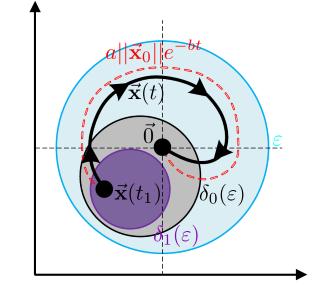
\includegraphics[width=0.5\textwidth]{figs/exponential-stability}
\vspace{-4pt}
\caption{Exponential stability, $\mathbf{UES}$}
\label{fig:exponential-stability}
\vspace{-6pt}
\end{figure}
\par
The above definitions of stability are only locally defined, and so the stabilities hold true only for local trajectories, only in the case of $\vec{\mathbf{x}}(t_0)\leq\varepsilon$. Extending \textbf{UAS} to global uniform asymptotic stability (\textbf{GUAS}); the origin's equilibrium point is \textbf{GUAS} \emph{iff} conditions for \textbf{UAS} are first met, the origin is only the equilibrium point and the asymptotic approach can be extended such that:
\begin{subequations}
\begin{equation}
\exists~\delta_1(\varepsilon)>0:~\norm{\vec{\mathbf{x}}(t_1)}<\delta_1(\varepsilon),~~t_1\geq t_0
\end{equation}
\vspace{-16pt}
\begin{equation}
\Rightarrow \lim_{t\rightarrow\infty}\norm{\vec{\mathbf{x}}(t)}\rightarrow \vec{0},~~\forall \vec{\mathbf{x}}(t_0)
\end{equation}
\end{subequations}
Similarly exponential stability can extend to the global case \emph{iff} \textbf{UES} conditions are first met. In the global case, the origin can be the only equilibrium point. Stability from Eq:\ref{eq:exponential-stability} is then globally:
\begin{equation}\label{eq:global-exponential-stability}
\norm{\vec{\mathbf{x}}(t,t_0)}\leq a\norm{\vec{\mathbf{x}}_0}e^{-bt},~~\forall\norm{\vec{\mathbf{x}}_0}
\end{equation}
Initial equilibrium point conditions are dropped in Eq:\ref{eq:global-exponential-stability}. It follows that, irrespective of the starting point for the trajectory, the system \underline{always} settles to the origin. \textbf{GUES} is the strongest sense of stability and further provides insight into the rate at which the trajectory stabilizes. The most desirable control design outcome is a controller which applies globally uniform exponential stability to a plant.
%====================================================
\section{Lyapunov Stability Theorem}
\label{sec:control.lyapunov}
%====================================================
Lyapunov's stability theory is an important aspect of non-linear control design. An abundance of literature exists on the subject, included in almost every meritable textbook or control paper. If the reader is unfamiliar with Lyapunov's theorem,  \cite{noteonlyapunov,nonlinearsystems,bojelayupanov} all explain in detail the concept. The following is adapted from \cite{bojelayupanov} and \cite{lyapunovstabilitytheorem} and briefly outlines how Lyapunov's stability theorem is used to prove (\emph{global}) asymptotic stability for continuous time invariant systems, linear or otherwise.
\par
The theory analyses a generalized energy function of a system's autonomous trajectory. If the trajectory has a negative energy derivative that implies the system's energy will always dissipate towards a stable equilibrium point. 
\par
Lyapunov analysis is a powerful method for stability verification, the system's trajectory itself need not be explicitly defined for stability to be ascertained. Proof of Lyapunov's theorem is done with a contradiction disproof and, as such, the theoretical underpinning is somewhat cumbersome.
\par
It's worth reiterating its fundamentals given that backstepping controllers are proposed later in Sec:\ref{subsec:control.attitude.nonlinear} for attitude control. A backstepping controller iteratively enforces Lyapunov stability criterion onto the system through the control structure, \cite{backstepping,adaptivebackstep,intelligentbackstep}. In general, given a non-linear time invariant system that follows some continually differentiable trajectory $\mathbf{x}(t)$, typically the trajectory is going to progress subject to some rule:
\begin{equation}
\dot{\mathbf{x}}(t)=f\big(\vec{\mathbf{x}}(t),u\big)
\end{equation}
Then, constructing a generalized positive-definite function (generalized energy or \emph{Lyapunov function candidate}) $V(\mathbf{x})$ for a trajectory $\mathbf{x}(t)$. A positive definite matrix, $M$, is defined such that:
\begin{equation}
\mathbf{z}^TM\mathbf{z}\geq 0~~~\forall \mathbf{z}
\end{equation}
As such an LFC typically, but not exclusively, has the quadratic and positive-definite form:
\begin{equation}
V(\mathbf{x})=\mathbf{x}^TP\mathbf{x}
\end{equation}
An LFC could simply be positive semi-definite over the trajectory's bound, the quadratic form is convenient for the use of backstepping. From its definition the trajectory is continually differentiable; there is then a gradient matrix for each component of $V(x)$ in the form:
\begin{equation}
\nabla V(\vec{\mathbf{x}})\triangleq\bigg[\frac{\partial V(\vec{\mathbf{x}})}{\partial x_1}~\frac{\partial V(\vec{\mathbf{x}})}{\partial x_2}~\ldots~\frac{\partial V(\vec{\mathbf{x}})}{\partial x_n}\bigg]~~~~\vec{\mathbf{x}}\in\mathbb{R}^n
\end{equation}
The energy function's derivative, otherwise referred to as the \emph{Lie derivative}\cite{noteonlyapunov,nonlinearsystems} is calculated as follows:
\begin{equation}
\dot{V}(\vec{\mathbf{x}})\triangleq\nabla V(\vec{\mathbf{x}})^T\frac{d}{dt}f(\vec{\mathbf{x}})=\frac{\delta V(x)}{\delta x_1}\frac{df_1(x)}{dt}+\frac{\delta V(x)}{\delta x_2}\frac{df_2(x_2)}{dt}+~\ldots~+\frac{\delta V(x)}{\delta x_n}\frac{df_n(x)}{dt}
\end{equation}
Lyapunov's theorem states that \emph{iff} the candidate function $V(\vec{\mathbf{x}})$ is positive definite with $V(\vec{0})=0$ and its derivative is strictly negative; $\dot{V}(\vec{\mathbf{x}})< 0~~\forall \vec{\mathbf{x}}(t) \not= 0$, the system is then asymptotically stable ($\mathbf{AS}$ from Eq:\ref{eq:asymptotic-stability}). Mathematically that means, for any $\vec{\mathbf{x}}(t)$ with $t\geq t_0$:
\begin{equation}
V\big(\vec{\mathbf{x}}(t)\big)=V\big(\vec{\mathbf{x}}(t_0)\big)+\int_{t_0}^t \dot{V}\big(\mathbf{x}(t)\big).dt \leq V\big(\mathbf{x}(t_0)\big)
\end{equation}
Which can be physically interpreted as the system's generalized energy function dissipating, irrespective of the trajectory path taken. With a strictly decreasing energy function, the system will stabilize to an equilibrium point. 
\begin{equation}
\lim_{t\rightarrow\infty}\norm{V\big(\vec{\mathbf{x}}(t)\big)}\rightarrow 0
\end{equation}
The trajectory's asymptotic stability can be extended to exponential stability boundedness, such that \emph{iff} the same conditions are met and there exists some positive coefficient $\alpha>0$ such that $\dot{V}(\vec{\mathbf{x}})\leq-\alpha V(\vec{\mathbf{x}})$. That implies the system is globally exponentially stable as is bound in such a way that:
\begin{equation}
\norm{V\big(\vec{\mathbf{x}}(t)\big)}\leq Me^{-\alpha t/2}\norm{V\big(\vec{\mathbf{x}}(t_0)\big)}
\end{equation}
%====================================================
\section{Model Dependent \& Independent Controllers}
%====================================================
Two classes of controllers are included for a full state trajectory tracking control loop; both attitude and position control laws. Attitude set-point tracking is the primary focus of this research project (Sec:\ref{subsec:control.attitude.problem}) and incorporates a more detailed schedule of controller design and evaluation. 
\par
The allocation law combines both virtual control inputs from attitude and position controllers, $\vec{\nu}_d=[\vec{F}_\mu(u)~\vec{\tau}_\mu(u)]^T$, to solve for explicit actuator positions. Controller dependency on the plant's state is as a consequence of the actuator responses and complex inertial dynamics, as derived previously in Sec:\ref{subsec:dynamics.nonlinearities.gyrotorques}. Whilst not a prerequisite for stability, plant dependent compensation obviously improves controller performances. Independent and dependent cases are only considered for one type of controller; the most basic case PD controller in Section:\ref{subsubsec:control.attitude.controllers.pd} and tested in Sec:\ref{subsec:simulation.attitude.pd}. All other control laws compensate for unwanted plant dynamics in a feedback configuration.
\par
The plant dependency makes backstepping controllers an effective controller choice for this dissertation's context. The proposed plant dependent control laws compensate for undesirable dynamics their design, basic PD and PID control structures (\emph{and the like}) will not. The first and most basic control solution, used as a reference case, is a PD controller for attitude and position with direct-inversion (Pseudo or Moore-Penrose inversion) allocation. 
%====================================================
\section{Attitude Control}
\label{sec:control.attitude}
%====================================================
\subsection{The Attitude Control Problem}
\label{subsec:control.attitude.problem}
%====================================================
The set-point tracking control problem (\cite{attitudecontrolproblem}) for the attitude plant is to design a stabilizing control torque $\vec{\tau}_d=h(\mathbf{x}_e,t)$ such that for any desired attitude quaternion, $\forall~Q_d\in\mathbb{Q}$, and an instantaneous attitude body quaternion, $Q_b(t)\in\mathbb{Q}$, the error state asymptotically stabilizes to the origin; $Q_e\rightarrow[1~\vec{0}~]^T$. Or that:
\begin{equation}
\vec{\tau}_d=h(Q_d,~\dot{Q}_d,~Q_b(t),~\dot{Q}_b(t))~~\text{such that}~~\underset{t\rightarrow\infty}{\lim}Q_b(t)\rightarrow Q_d
\end{equation}
Quaternion attitude error states are defined as the Hamilton product (\emph{difference}) between the desired and instantaneous quaternion attitude states. Quaternion error states are multiplicative, in contrast with the subtractive relationship for Euler angle error states. The attitude error state is calculated as:
\begin{equation}\label{eq:quaternion-error}
Q_e\triangleq Q_b^*(t)\otimes Q_d
\end{equation}
The relative angular velocity error between the body frame, $\mathcal{F}^b$, and the trajectory's desired frame, $\mathcal{F}^d$, is given as $\vec{\omega}_e$. The body angular velocity, $\vec{\omega}_b$ is subject to the differential Eq:\ref{eq:quaternion-states-angular}. As such there is an angular rate error:
\begin{subequations}
\begin{equation}\label{eq:angular-error}
\vec{\omega}_e\triangleq\vec{\omega}_d-\vec{\omega}_b(t)
\end{equation}
The desired angular velocity is taken with respect to the desired angular attitude frame, and so it must be transformed back onto the existing body frame.
\begin{equation}
\vec{\omega}_e=Q_e^*\otimes\vec{\omega}_d\otimes Q_e-\vec{\omega}_b(t)
\end{equation}
Typically for the trajectories generated here the desired angular velocity is zero; $\vec{\omega}_d=\vec{0}$. It follows that the angular rate error is then simply the negative body angular velocity. It would be easy to incorporate a non-zero angular velocity setpoint to accommodate for higher order state derivative tracking trajectories.
\begin{equation}
\vec{\omega}_e=-\vec{\omega}_b(t)\Big|_{\vec{\omega}_d=\vec{0}}
\end{equation}
\end{subequations}
The time derivative of the quaternion error state is calculated from the quaternion derivative definition Eq:\ref{eq:quaternion-deriv}. The derivative $\dot{Q}_e$ is then dependent on the angular velocity error and calculated as follows:
\begin{equation}
\dot{Q}_e=\frac{1}{2}Q_e\otimes\vec{\omega}_e=-\frac{1}{2}Q_e\otimes\vec{\omega}_b(t)\Big|_{\vec{\omega}_d=\vec{0}}
\end{equation}
%====================================================
\subsection{Linear Controllers}
\label{subsec:control.attitude.controllers}
%====================================================
\subsubsection{PD Controller}
\label{subsubsec:control.attitude.controllers.pd}
%====================================================
The following control law is used as a reference case for comparison of the remaining controllers derived. It is a simple Proportional-Derivative attitude controller, adapted from \cite{fullquaternion} and following a stability proof similar to the one derived in \cite{attitudecontrolproblem}. An attitude PD controller is proportional only to the vector quaternion error. Such that the error is the same dimension as the angular velocity error; $\in\mathbb{R}^3$. A PD controller designs the control torque as:
\begin{equation}\label{eq:independent-pd}
\vec{\tau}_{_{PD}}=K_d\vec{\omega}_e+K_p\vec{q}_e~~~~[Nm],~\in\mathcal{F}^b
\end{equation}
Where both $K_d$ and $K_p$ are positive definite symmetrical $3\times 3$ coefficient matrices to be determined later. Eq:\ref{eq:independent-pd} neglects the quaternion scalar error and is therefore susceptible to unwinding. Using a positive-definite Lyapunov function candidate $V_{_{PD}}$ for the attitude trajectory:
\begin{equation}\label{eq:lyapunov-pd}
V_{_{PD}}(\vec{q}_e,\vec{\omega}_e)=K_p\vec{q}_e\text{}^T\vec{q}_e+K_p(|q_0|-1)^2+\frac{1}{2}\vec{\omega}_e\text{}^TJ_b(u)\vec{\omega}_e
\end{equation}
Recalling the angular velocity differential equation from Eq:\ref{eq:quaternion-states-angular}, $\dot{\vec{\omega}}_b$ is:
\begin{equation}
\dot{\vec{\omega}}_b=J_b\text{}^{-1}(u)\big(-\vec{\omega}_b\times J_b(u)\vec{\omega}_b-\hat{\tau}_b(u)+\vec{\tau}_g+\vec{\tau}_Q+\vec{\tau}_\mu(u)\big)~~~~\in\mathcal{F}^b
\end{equation}
Where $\vec{\tau}_Q$ is a simplified representation of the net aerodynamic torque experienced by the body from the rotating propellers, drawn from Eq:\ref{eq:aerodynamic-torque}. Then, exploiting a unit quaternion's inherent property, it follows that:
\begin{equation}\label{eq:4.17}
\norm{Q}=\vec{q}\text{}^{\hspace{3pt}T}\vec{q}+q_0\text{}^2=\vec{q}\text{}^{\hspace{3pt}2}+q_0\text{}^2=1
\end{equation}
Substituting the angular velocity error state, $\vec{\omega}_e=-\vec{\omega}_b$, the proportional derivative LFC in Eq:\ref{eq:lyapunov-pd} is simplified:
\begin{subequations}\label{eq:4.18}
\begin{equation}
V_{_{PD}}=K_p\vec{q}_e\text{}^2+K_p\big(|q_0|\text{}^2 -2|q_0|\big) + 1 +\frac{1}{2}\vec{\omega}_e\text{}^TJ_b(u)\vec{\omega}_e
\end{equation}
\vspace{-10pt}
\begin{equation}
=2K_p(1-|q_0|)+\frac{1}{2}\vec{\omega}_b\text{}^TJ_b(u)\vec{\omega}_b
\end{equation}
\end{subequations}
Similarly, using the fact that a quaternion's derivative is defined as:
\begin{equation}\label{eq:quat-derivative}
\dot{Q}=\begin{bmatrix}
-\frac{1}{2}\vec{q}^{\hspace{3pt}T}\vec{\omega}\\
\frac{1}{2}\big([\vec{q}]_\times+q_0\mathbb{I}_{3\times 3}\big)\vec{\omega}
\end{bmatrix}
\end{equation}
Substituting the above into the LFC derivative, $\dot{V}_{_{PD}}$, yields:
\begin{subequations}
\begin{equation}
\dot{V}_{_{PD}}=2K_p\frac{1}{2}\vec{q}_e\text{}^T\vec{\omega}_e+\frac{1}{2}\dot{\vec{\omega}}_b\text{}^TJ_b(u)\vec{\omega}_b+\frac{1}{2}\vec{\omega}_bJ_b(u)\dot{\vec{\omega}}_b\text{}^T
\end{equation}
\vspace{-12pt}
\begin{equation}
=-K_p\vec{q}_e\text{}^T\vec{\omega}_b+\vec{\omega}_b\text{}^TJ_b(u)\dot{\vec{\omega}}_b
\end{equation}
\end{subequations}
Expanding the angular acceleration $\dot{\vec{\omega}}_b$ and introducing the PD control law from Eq:\ref{eq:independent-pd}, $\vec{\tau}_{_{PD}}$ substituted back into the LFC derivative:
\begin{subequations}
\begin{equation}
\rightarrow\dot{V}_{_{PD}}=-K_p\vec{q}_e\text{}^T\vec{\omega}_b+\vec{\omega}_b\text{}^T\big(-\vec{\omega}_b\times J_b(u)\vec{\omega}_b-\hat{\tau}_b+\vec{\tau}_g+\vec{\tau}_Q-K_d\vec{\omega}_b+K_p\vec{q}_e\big)
\end{equation}
\vspace{-10pt}
\begin{equation}
=-K_p\vec{q}_e\text{}^T\vec{\omega}_b+K_p\vec{\omega}_b\text{}^T\vec{q}_e-\vec{\omega}_b\text{}^TK_d\vec{\omega}_b+\vec{\omega}_b\text{}^T\big(-\vec{\omega}_b\times J_b(u)\vec{\omega}_b-\hat{\tau}_b+\vec{\tau}_g+\vec{\tau}_Q\big)
\end{equation}
It follows that the transpose term $\vec{q}_e\text{}^T\vec{\omega}_b\iff\vec{\omega}_b\text{}^T\vec{q}_e$ is interchangeable as its resultant product is the same. The LCF derivative then simplifies:
\begin{equation}
\therefore\dot{V}_{_{PD}}=-\vec{\omega}_b\text{}^TK_d\vec{\omega}_b+\vec{\omega}_b\text{}^T\big(-\vec{\omega}_b\times J_b(u)\vec{\omega}_b-\hat{\tau}_b+\vec{\tau}_g+\vec{\tau}_Q\big)
\end{equation}
\end{subequations}
Then, as long as $\big(-\vec{\omega}_b\times J_b(u)\vec{\omega}_b-\hat{\tau}_b+\vec{\tau}_g+\vec{\tau}_Q\big)\leq \vec{0}$, some basic stability is guaranteed. Under specific circumstances the following assumptions can be made to ensure the asymptotic stability proof can be applied. The stability obviously breaks down if any of the assumptions fail, as such the stability is not global\ldots
\vspace{-10pt}
\begin{enumerate}[itemsep=0em]
\item The inertial matrix, $J_b(u)$, is approximately diagonal which, given the inertia ranges from Eq:\ref{eq:inertia-max} and Eq:\ref{eq:inertia-min}, is reasonable. Similarly that the angular rate can be made small with appropriately slow trajectory updates such that the torque gyroscopic cross-product is negligible:
\begin{center}
\vspace{-10pt}
$\vec{\omega}_b^{~T}\big(\vec{\omega}_b\times J_b(u)\vec{\omega}_b\big)\approx\vec{0}$
\vspace{-8pt}
\end{center}
\item The actuator rate torque response, $\hat{\tau}_b(u)$, is a second order effect dependent on $\dot{u}$. Typically the actuator rates are going to be kept small, Fig:\ref{fig:tau-body} shows torques $\hat{\tau}_b(u)$ for a typical trajectory. For slow attitude steps those position changes are small enough to be considered negligible. The approximation is made:
\begin{center}
\vspace{-10pt}
$\hat{\tau}_b(u)\approx\vec{0}$
\vspace{-8pt}
\end{center}
\item Finally, for the sake of the stability proof, the eccentric gravitational torque arm is neglected, $\vec{\tau}_g\approx\vec{0}$. Such a situation only holds true if $u\approx\vec{0}$ or that servo actuator positions are close to their zero positions.
\end{enumerate}
{\emph{\color{Gray}All of the above assumptions are made under extraneous circumstances and can not be assumed for almost all of the prototype's flight envelope. The plant independent case is considered and simulated in Sec\ref{subsubsec:simulation.atttiude.pd.independent} purely for contrition; mainly to demonstrate the need for plant dependent compensation.}
\par
If each of the assumptions made hold true, then the Lyapunov function's derivative is approximately negative definite. The stability proof for a very local trajectory is then:
\begin{subequations}
\begin{equation}
\dot{V}_{_{PD}}\approx-K_p\vec{q}_e\text{}^T\vec{\omega}_b+\vec{\omega}_b\text{}^T\big(-K_d\vec{\omega}_b+K_p\vec{q}_e\big)
\end{equation}
\vspace{-14pt}
\begin{equation}\label{eq:pd-local-stability}
\rightarrow\dot{V}_{_{PD}}=-\vec{\omega}_b\text{}^TK_d\vec{\omega}_b=-K_d\norm{\vec{\omega}_b}\text{}^2<0
\end{equation}
\end{subequations}
From Lyapunov stability theorem there then exists the limits for \emph{local} asymptotic stability: 
\begin{subequations}
\begin{equation}
\lim_{t\rightarrow\infty}\vec{\omega}_e\rightarrow\vec{0}~~\therefore~~\lim_{t\rightarrow\infty}\vec{\omega}_b\rightarrow\vec{0}^{-}
\end{equation}
\vspace{-14pt}
\begin{equation}
\lim_{t\rightarrow\infty}\vec{q}_e\rightarrow \vec{0}~~\text{and}~~\lim_{t\rightarrow\infty}(1-q_0)\rightarrow 0
\end{equation}
\end{subequations}
Hence the quaternion error stabilizes $Q_e\rightarrow[1~\vec{0}\hspace{3pt}]^{T}$ as $t\rightarrow\infty$. The stability shown in Eq:\ref{eq:pd-local-stability} is only local; introducing plant dependent compensation to the PD control law in Eq:\ref{eq:independent-pd} alleviates the stringent requirements on assumptions 1 through 3. Obviously compensation terms are \emph{state estimates} and so a small degree of uncertainty exists (stability is discussed in Sec:\ref{subsec:simulation.comparison.attitude}):
\begin{equation}\label{eq:dependent-pd}
\vec{\tau}_{_{PD}}=\vec{\omega}_b\times J_b(u)\vec{\omega}_b+\hat{\tau}_b(u)-\vec{\tau}_g-\vec{\tau}_Q+K_d\vec{\omega}_e+K_p\vec{q}_e
\end{equation}
The resultant stability proof for the plant dependent case Eq:\ref{eq:dependent-pd} is much the same as that for the independent controller, Eq:\ref{eq:independent-pd}. The same LCF from Eq:\ref{eq:lyapunov-pd} shows that Eq:\ref{eq:pd-local-stability} holds for all global trajectories:
\begin{equation}\label{eq:dependent-global-stability}
\rightarrow\dot{V}_{_{PD}}=-\vec{\omega}_b\text{}^TK_d\vec{\omega}_b=-K_d\norm{\vec{\omega}_b}\text{}^2<\vec{0}~~\forall(Q_e,\vec{\omega}_b)
\end{equation}
A plant dependent controller is not reliant on the very limiting assumptions needed for independent asymptotic stability to be achieved. The dynamic compensation in Eq:\ref{eq:dependent-pd} is simple to implement; especially considering the form of unwanted dynamics which have already quantified and corroborated previously in Sec:\ref{subsec:dynamics.nonlinearities.torque-tests}.
%====================================================
\subsubsection{Auxiliary Plant Controller}
\label{subsubsec:control.attitude.controllers.auxpd}
%====================================================
Expanding on what has, in practice (Table:\ref{tab:controllers}, Sec:\ref{subsec:intro.lit.related}), proven to be a popular and effective controller for attitude stabilization, \cite{attitudestabilization} proposed an auxiliary plant term to a P-D attitude controller. Most significantly, the altered PD controller adds auxiliary terms proportional to the quaternion rate error (Eq:\ref{eq:quaternion-deriv}). Moreover part of the auxiliary plant is proportional to the \emph{quaternion scalar} $q_0$, a term that is otherwise neglected in the previous PD control law (Sec:\ref{subsubsec:control.attitude.controllers.pd}) and prevents unwinding if incorporated. The \emph{auxilliarly} PD control torque is a function of errors states:
\begin{equation}\label{eq:control-aux-pd}
\vec{\tau}_{_{XPD}}=\underbrace{-\Gamma_2{\widetilde{\Omega}}-\Gamma_3\vec{q}_e+J_b(u)\dot{\bar{\Omega}}}_{Independent}+\underbrace{\vec{\omega}_b\times J_b(u)\vec{\omega}_b+\hat{\tau}_b-\vec{\tau}_g-\vec{\tau}_Q}_{Compensation}
\end{equation}
Wherein the coefficients $\Gamma_2$ and $\Gamma_3$ are both diagonal positive definite coefficient matrices whilst $\Gamma_1$, used next in Eq:\ref{eq:aux-pd-1}, is a symmetrical matrix. Each coefficient matrix is explicitly determined later. Auxiliary plants $\widetilde{\Omega}$ and $\dot{\bar{\Omega}}$ are defined as follows. The first auxiliary plant $\bar{\Omega}$ is proportional to the quaternion error and hence its derivative $\dot{\bar{\Omega}}$ is a quaternion rate:
\begin{subequations}\label{eq:aux-pd-1}
\begin{equation}
\bar{\Omega}\triangleq-\Gamma_1\vec{q}_e~~\therefore~~\dot{\bar{\Omega}}=-\Gamma_1\dot{\vec{q}}_e
\end{equation}
\vspace{-15pt}
\begin{equation}
\rightarrow\dot{\bar{\Omega}}=-\frac{1}{2}\Gamma_1\big(q_0\mathbb{I}_{3X3}+[\vec{q}_e]_{\times}\big)\vec{\omega}_e
\end{equation}
\vspace{-10pt}
\begin{equation}
=\frac{1}{2}\Gamma_1\big(q_0\mathbb{I}_{3X3}+[\vec{q}_e]_{\times}\big)\vec{\omega}_b\Big|_{\vec{\omega}_e=-\vec{\omega}_b}
\end{equation}
\end{subequations}
The second auxiliary plant, $\widetilde{\Omega}$, is proportional to both quaternion vector and angular velocity errors.
\begin{subequations}\label{eq:aux-pd-2}
\begin{equation}
\widetilde{\Omega}\triangleq\vec{\omega}_e-\bar{\Omega}=\vec{\omega}_e+\Gamma_1\vec{q}_e
\end{equation}
\vspace{-15pt}
\begin{equation}
=-\vec{\omega}_b+\Gamma_1\vec{q}_e\Big|_{\vec{\omega_e}=-\vec{\omega}_b}
\end{equation}
\end{subequations}
Using an LFC similar to the basic $V_{_{PD}}$ function candidate from Eq:\ref{eq:lyapunov-pd}, but substituting an auxiliary term $\widetilde{\Omega}$ for the body's angular velocity $\vec{\omega}_b$ into the LFC $V_{_{XPD}}$:
\begin{equation}\label{eq:lyapunov-xpd}
V_{_{XPD}}\big(\vec{q}_e,~\widetilde{\Omega}\big)=\vec{q}_e\text{}^T\vec{q}_e+\big(|q_0|-1\big)^2+\frac{1}{2}\widetilde{\Omega}\text{}^{\hspace{1pt}T}\big(\Gamma_3^{-1}J_b(u)\big)\widetilde{\Omega}
\end{equation}
Again using the simplification from a quaternion's inherent properties in Eq:\ref{eq:4.17}, the LFC from Eq:\ref{eq:lyapunov-xpd} then simplifies with the following derivative:
\begin{subequations}
\vspace{-5pt}
\begin{equation}
V_{_{XPD}}=2(1-|q_0|)+\frac{1}{2}\widetilde{\Omega}\text{}^{\hspace{1pt}T}\big(\Gamma_3^{-1}J_b(u)\big)\widetilde{\Omega}
\end{equation}
\vspace{-11pt}
\begin{equation}
\dot{V}_{_{XPD}}=2\frac{1}{2}\vec{q}_e\text{}^T\vec{\omega}_e+\frac{1}{2}\dot{\widetilde{\Omega}}\text{}^{\hspace{1pt}T}\big(\Gamma_3^{-1}J_b(u)\big)\widetilde{\Omega}+\frac{1}{2}\widetilde{\Omega}\text{}^{\hspace{1pt}T}\big(\Gamma_3^{-1}J_b(u)\big)\dot{\widetilde{\Omega}}
\end{equation}
\vspace{-8pt}
\begin{equation}\label{eq:4.34c}
\dot{V}_{_{XPD}}=-\vec{q}_e\text{}^T\vec{\omega}_b+\frac{1}{2}\dot{\widetilde{\Omega}}\text{}^{\hspace{1pt}T}\big(\Gamma_3^{-1}J_b(u)\big)\widetilde{\Omega}+\frac{1}{2}\widetilde{\Omega}\text{}^{\hspace{1pt}T}\big(\Gamma_3^{-1}J_b(u)\big)\dot{\widetilde{\Omega}}\Big|_{\vec{\omega}_e=-\vec{\omega}_b}
\end{equation}
\end{subequations}
It then follows, substituting $\dot{\vec{\omega}}_b$ from Eq:\ref{eq:aux-pd-2}, the auxiliary plant's derivative $\dot{\widetilde{\Omega}}$ is:
\begin{subequations}
\vspace{-6pt}
\begin{equation}
\dot{\widetilde{\Omega}}=-\dot{\vec{\omega}}_b+\Gamma_1\dot{\bar{\Omega}}
\end{equation}
\vspace{-15pt}
\begin{equation}
\rightarrow\dot{\vec{\omega}}_b=J_b^{-1}(u)\big(-\vec{\omega}_b\times J_b(u)\vec{\omega}_b-\hat{\tau}_b+\vec{\tau}_g+\vec{\tau}_Q+\vec{\tau}_{_{XPD}}\big)
\end{equation}
\vspace{-10pt}
\begin{equation}
\therefore\dot{\widetilde{\Omega}}=-J_b^{-1}(u)\big(-\vec{\omega}_b\times J_b(u)\vec{\omega}_b-\hat{\tau}_b+\vec{\tau}_g+\vec{\tau}_Q+\vec{\tau}_{_{XPD}}\big)-\Gamma_1\dot{\bar{\Omega}}
\end{equation}
Substituting the auxiliary PD control law, $\vec{\tau}_{_{XPD}}$ from Eq:\ref{eq:control-aux-pd}, into the auxiliary derivative $\dot{\widetilde{\Omega}}$:
\begin{equation}
\rightarrow\dot{\widetilde{\Omega}}=J_b^{-1}(u)\big(J_b(u)\dot{\bar{\Omega}}-\Gamma_2\widetilde{\Omega}-\Gamma_3\vec{q}_e\big)-\dot{\bar{\Omega}}
\end{equation}
\vspace{-15pt}
\begin{equation}
=J_b^{-1}(u)\big(-\Gamma_2\widetilde{\Omega}-\Gamma_3\vec{q}_e\big)
\end{equation}
\end{subequations}
From the \emph{approximately} diagonal inertial matrix $J_b(u)$ and the positive symmetric (or \emph{diagonal}) properties of the coefficient matrices $\Gamma_1$,$\Gamma_2$ and $\Gamma_3$; the auxiliary plant $\dot{\widetilde{\Omega}}$ has a transpose:
\begin{equation}
\dot{\widetilde{\Omega}}\text{}^{\hspace{1pt}T}=J_b^{-1}\big(-\Gamma_2\widetilde{\Omega}^{\hspace{1pt}T}-\Gamma_3\vec{q}_e\text{}^T\big)
\end{equation}
The PD auxiliary plant component(s) in the LFC derivative $\dot{V}_{_{XPD}}$ in Eq:\ref{eq:lyapunov-xpd} simplifies:
\begin{subequations}
\begin{equation}
\frac{1}{2}\dot{\widetilde{\Omega}}\text{}^{\hspace{1pt}T}\big(\Gamma_3^{-1}J_b(u)\big)\widetilde{\Omega}=\frac{1}{2}\big(-\Gamma_2\widetilde{\Omega}\text{}^{\hspace{1pt}T}-\Gamma_3\vec{q}_e\text{}^T\big)\Gamma_3^{-1}\widetilde{\Omega}
\end{equation}
\vspace{-12pt}
\begin{equation}\label{eq:4.48b}
=\frac{1}{2}\big(-\widetilde{\Omega}\text{}^{\hspace{1pt}T}\Gamma_2\Gamma_3^{-1}\widetilde{\Omega}-\vec{q}_e\text{}^{T}\widetilde{\Omega}\big)
\end{equation}
Substituting Eq:\ref{eq:aux-pd-2} for $\vec{q}_e\text{}^T\widetilde{\Omega}$ into Eq:\ref{eq:4.48b}:
\begin{equation}\label{eq:4.48c}
\rightarrow\frac{1}{2}\dot{\widetilde{\Omega}}^T\big(\Gamma_3^{-}J_b(u)\big)\widetilde{\Omega}=\frac{1}{2}\big(-\widetilde{\Omega}\text{}^{\hspace{1pt}T}\Gamma_2\Gamma_3^{-1}\widetilde{\Omega}+\vec{q}_e\text{}^T\vec{\omega}_b-\vec{q}_e\text{}^T\Gamma_1\vec{q}_e\big)\Big|_{\vec{q}_e\text{}^{T}\widetilde{\Omega}=-\vec{q}_e\text{}^{T}\vec{\omega}_b+\Gamma_1\vec{q}_e\text{}^{T}}
\end{equation}
Similarly, for the transposed counterpart of Eq:\ref{eq:4.48c} in Eq:\ref{eq:4.34c}:
\begin{equation}
\frac{1}{2}\widetilde{\Omega}\text{}^{\hspace{1pt}T}\big(\Gamma_3^{-1}J_b(u)\big)\dot{\widetilde{\Omega}}=\frac{1}{2}\big(-\widetilde{\Omega}\Gamma_2\Gamma_3^{-1}\widetilde{\Omega}\text{}^{\hspace{1pt}T}+\vec{q}_e\vec{\omega}_b\text{}^T-\vec{q}_e\Gamma_1\vec{q}_e\text{}^T\big)
\end{equation}
Which, when substituted back into Eq:\ref{eq:4.34c}, then simplifies the LFC derivative to negative definite:
\end{subequations}
\begin{equation}
\Rightarrow\dot{V}_{_{XPD}}=-\vec{q}_e\text{}^T\Gamma_1\vec{q}_e-\widetilde{\Omega}\Gamma_2\Gamma_3^{-1}\widetilde{\Omega}\text{}^{\hspace{1pt}T}<0~~~~\forall~(\vec{q}_e,\widetilde{\Omega})
\end{equation}
As such, the control law $\vec{\tau}_{_{XPD}}$ asymptomatically stabilizes the attitude plant globally. Both $\widetilde{\Omega}$ and $\vec{q}_e$ tend to $\vec{0}$, or more specifically the following global stability limits exist:
\begin{subequations}
\begin{equation}
\underset{t\rightarrow\infty}{\lim}\vec{q}_e=0~~\text{and}~~\underset{t\rightarrow\infty}{\lim}\widetilde{\Omega}=0
\end{equation}
Then, from the auxiliary plant definition(s) in Eq:\ref{eq:aux-pd-2}, the extended limits present themselves;
\begin{equation}
\underset{t\rightarrow\infty}{\lim}\vec{\omega}_b=\vec{0}\Big|_{\vec{\omega}_d=\vec{0}}~~~\text{and}~~~\underset{t\rightarrow\infty}{\lim}\bar{\Omega}=\vec{0}
\end{equation}
\end{subequations}
Whilst global asymptotic stability is indeed satisfactory, faster exponential stability is obviously more desirable. The stability proof for $V_{_{XPD}}$ can be extended to a stable exponentially bounded trajectory. From a quaternion's inherent definition it follows that $0\leq |q_0| \leq 1$. It can then be stated that:
\begin{equation}\label{eq:4.34}
1-|q_0|\leq 1-q_0^2=\norm{\vec{q}_e}^2
\end{equation}
Exponential stability is a maximum boundedness proof; the relationship Eq:\ref{eq:4.34} can then replace the quaternion scalar term $2(1-|q_0|)$ in $V_{_{XPD}}$ as an upper bound. The LFC is then rewritten in terms of its component's norm(s) to produce a bounding inequality:
\begin{subequations}\label{eq:xpd-ibc}
\begin{equation}
V_{_{XPD}}=\vec{q}_e\text{}^T\vec{q}_e+(|q_0|-1)^2+\frac{1}{2}\widetilde{\Omega}\text{}^{\hspace{1pt}T}\big(\Gamma_3^{-1}J_b(u)\big)\widetilde{\Omega}
\end{equation}
\vspace{-10pt}
\begin{equation}
\rightarrow V_{_{XPD}}\leq 2\norm{\vec{q}_e}\text{}^2+\frac{1}{2}\Gamma_3^{-1}J_b(u)||\widetilde{\Omega}||\text{}^2
\end{equation}
Similarly the LFC's derivative can be written in terms of its norms as:
\begin{equation}
\dot{V}_{_{XPD}}\leq-\Gamma_2\Gamma_3^{-1}||\widetilde{\Omega}||\text{}^2-\Gamma_1\norm{\vec{q}_e}\text{}^2
\end{equation}
\end{subequations}
The LFC, $V_{_{XPD}}$, has a maximum such that:
\begin{equation}
V_{_{XPD}}\leq max \bigg\{ 2,\frac{\lambda_{max}(\Gamma_3^{-1}J_b(u))}{2}\bigg\}\big(\norm{\vec{q}_e}\text{}^2+||\widetilde{\Omega}||\text{}^2\big)
\end{equation}
Where the function $\lambda_{max}$ represents the maximum eigenvalue of its argument; in this case $\Gamma_3^{-1}J_b(u)$. Similarly the \emph{negative definite} LCF derivative is bound by the minimum:
\begin{equation}
\dot{V}_{_{XPD}} \leq -min \big\{ \lambda_{min}(\Gamma_1),\lambda_{min}(\Gamma_2\Gamma_3\text{}^{-1})\big\}\big(\norm{\vec{q}_e}\text{}^2+||\widetilde{\Omega}||^2 \big)
\end{equation}
Therefore there exists some ratio $\alpha>0$ that satisfies the relationship requirement between the LCF and its derivative; $\dot{V}_{_{XPD}}\leq -\alpha V_{_{XPD}}$, where $\alpha$ is defined as the ratio:
\begin{equation}
\alpha=\frac{min\big\{\lambda_{min}(\Gamma_1),\lambda_{min}(\Gamma_2\Gamma_3\text{}^{-1})\big\}}{max\big\{2,\frac{\lambda_{max}(\Gamma_3\text{}^{-1}J_b(u))}{2}\big\}}
\end{equation}
The attitude trajectory $\big(\vec{q}_e(t),\widetilde{\Omega}(t)\big)$ is then exponentially bounded by:
\begin{equation}\label{eq:exponential-pd}
\big(\norm{\vec{q}_e(t)},||\widetilde{\Omega}(t)||\big)\leq Me^{-\alpha t/2}\big(\norm{\vec{q}_e(0)},||\widetilde{\Omega}(0)||\big)
\end{equation}
The bounding exponential coefficient $\alpha$ can be found using maximum Eigen values for the maximum inertia $J_b(u_{\Lambda})$ from Eq:\ref{eq:inertia-max}. Using the relationship in Eq:\ref{eq:exponential-pd} and testing proposed controller coefficients for $\Gamma_1,~\Gamma_2,~\Gamma_3$ the settling rate can be optimized.
\par
\emph{\color{Gray}The above stability proof for the auxiliary attitude controller was expanded upon and derived from \cite{attitudestabilization}, adapted to fit attitude setpoint tracking. Introduction of the quaternion error, which is dependent on the quaternion scalar, dramatically improves controller performance. The exponential stability notably improves settling times and overshoot errors, demonstrated in Sec:\ref{subsec:simulation.attitude.xpd}.}
\newpage
Interestingly a previously \cite{robustattitude} was the precursor for PD based attitude plants with asymptotic exponential stability. That proposed control law first did not make use of any defined \emph{auxiliary plants}, unlike Eq:\ref{eq:control-aux-pd}; however equivalent terms were effectively incorporated. The control law was developed for spacecraft attitude tracking and proposed a very similar exponentially stabilizing control scheme to that of $\vec{\tau}_{_{XPD}}$. That controller, when changed to the notational convention used above, designs body torque as:
\begin{equation}\label{eq:control-auxp-pd}
\vec{\tau}^{\hspace{3pt}'}_{_{XPD}}=-\frac{1}{2}\Big[\big([\vec{q}_e]_\times+q_0\mathbb{I}_{3\times 3}\big)\Gamma_1+\alpha\big(1-q_0\mathbb{I}_{3\times 3}\big)\Big]\vec{q}_e-\Gamma_2\vec{\omega}_b\in\mathcal{F}^b
\end{equation} 
Eq:\ref{eq:control-auxp-pd} could easily incorporate plant dependent compensation to accomodate for unwanted non-linear dynamics. Both exponentially stabilizing PD controllers, from Eq:\ref{eq:control-aux-pd} and above Eq:\ref{eq:control-auxp-pd}, bear a striking similarity to the ideal backstepping controllers derived next in Eq:\ref{eq:control-ibc}. 
%====================================================
\subsection{Non-linear Controllers}
\label{subsec:control.attitude.nonlinear}
%====================================================
Backstepping controllers(\cite{satellitebackstepping,intelligentbackstep,backstepslidingmode},etc\ldots) are a popular choice for non-linear attitude control plants. The process, through iterative design, enforces Lyapunov stability criteria to ensure asymptotic stability. A report, \cite{backstepping}, surveys the fundamentals of backstepping procedure. Ideal backstepping control (\emph{IBC}) is a precise control solution which requires exact plant matching, something that is difficult to achieve in practice. Considering that some state estimate, $\hat{\mathbf{x}}(t)$ is used for feedback control. The caveat of IBC control is poor robust stability performance; being especially susceptible to state dependent uncertainty. Unmodelled disturbances could easily drive the energy function away from stability conditions. The ideal backstepping algorithm can then be extended to incorporate such uncertainties. Adatively including disturbance and \emph{estimate} uncertainty into the LFC energy function improves the stability's robustness (Adaptive backstepping control, \emph{ABC}). By Lyapunov's theorem the respective estimation error terms are stabilized.
%====================================================
\subsubsection{Ideal Backstepping Controller}
\label{subsubsec:control.attitude.nonlinear.idealbackstep}
%====================================================
Starting with the ideal case for the first proposed backstepping controller, similar to \cite{satellitebackstepping}; it is assumed the attitude plant described in Eq:\ref{eq:quaternion-states-angular} from the consolidated model in Sec:\ref{sec:dynamics.model} exactly matches the dynamics of the physical prototype. The ideal backstepping controller aims to compensate for the plant's dynamic response to trajectory inputs perfectly. Neglecting uncertainties associated with the dynamic model, the aim here is to apply a stabilizing torque design. Recalling the quaternion tracking error from Eq:\ref{eq:quaternion-error}; $Q_e=Q_b^*\otimes Q_e$, considering the first LFC proposal:
\begin{equation}\label{eq:ibc-lfc-1}
V_1(\vec{q}_e)=\vec{q}_e\text{}^T\vec{q}_e+(|q_0|-1)^2
\end{equation}
The absolute $|q_0|$ quaternion scalar is applied to ensure global stability. After substituting in the quaternion derivatives and \emph{without} using the quaternion simplification in Eq:\ref{eq:4.18}, has a Lie derivative:
\begin{subequations}
\begin{equation}
\dot{V}_1=2\vec{q}_e\text{}^T\frac{1}{2}\big([\vec{q}_e]_\times+q_0\mathbb{I}_{3X3}\big)\vec{\omega}_e-2\big(q_0-1\big)\frac{1}{2}\vec{q}_e\text{}^T\vec{\omega}_e
\end{equation}
\vspace{-5pt}
\begin{equation}
=\vec{q}_e\text{}^T\big([\vec{q}_e]_\times+q_0\mathbb{I}_{3X3}\big)\vec{\omega}_e-q_0\vec{q}_e\text{}^T\vec{\omega}_e+\vec{q}_e\text{}^T\vec{\omega}_e
\end{equation}
Simplifying and then substituting $\vec{\omega}_e=\vec{\omega}_d-\vec{\omega}_b=\vec{0}-\vec{\omega}-b$:
\begin{equation}
=\vec{q}_e\text{}^T[\vec{q}_e]_\times\vec{\omega}_e+\vec{q}_e\text{}^T\vec{\omega}_e
\end{equation}
\vspace{-10pt}
\begin{equation}
=-\vec{q}_e\text{}^T[\vec{q}_e]_\times\vec{\omega}_b-\vec{q}_e\text{}^T\vec{\omega}_b\Big|_{\vec{\omega}_e=-\vec{\omega}_b}
\end{equation}
\end{subequations}
Then choosing the first virtual backstepping control input $\gamma_d$. Note that $\gamma_d$ is used here to \emph{differentiate the backstepping design value} from the trajectory commanded $\vec{\omega}_d$, Eq:\ref{eq:angular-error}. Choosing $\gamma_d$ such that the first LFC Eq:\ref{eq:ibc-lfc-1} is negative definite, $\dot{V}_1<0$:
\begin{equation}
\vec{\omega}_b\Rightarrow\gamma_d=\Gamma_1\vec{q}_e
\end{equation}
Where $\Gamma_1$ is the first symmetric positive definite gain matrix, a fact that is important to stress due to positive definite matrix's invertability. That backstepping input simplifies the LFC derivative $\dot{V}_1$ to the negative definite term:
\begin{subequations}
\begin{equation}
\dot{V}_1=-\vec{q}_e\text{}^T[\vec{q}_e]_\times\gamma_d-\vec{q}_e\text{}^T\gamma_d
\end{equation}
\vspace{-14pt}
\begin{equation}
=-\vec{q}_e\text{}^T[\vec{q}_e]_\times\Gamma_1\vec{q}_e-\vec{q}_e\text{}^T\Gamma_1\vec{q}_e
\end{equation}
And considering a vector cross product with itself has a zero resultant, $\vec{q}_e\text{}^T[\vec{q}_e]_\times=\vec{0}$, $\dot{V}_1$ then reduces:
\begin{equation}
=-\vec{q}_e\text{}^T\Gamma_1\vec{q}_e<0
\end{equation}
\end{subequations}
However, that backstepping input $\gamma_d$ has its own associated error. A stabilizing law $z_1$ needs to control that error:
\begin{subequations}
\begin{equation}
z_1\triangleq\vec{\omega}_b-\gamma_d=\vec{\omega}_b-\Gamma_1\vec{q}_e\Big|_{\gamma_d=\Gamma_1\vec{q}_e}
\end{equation}
\vspace{-8pt}
\begin{equation}
\rightarrow\vec{\omega}_b=z_1+\Gamma_1\vec{q}_e
\end{equation}
\vspace{-10pt}
\begin{equation}
\therefore\dot{V}_1=-\vec{q}_e\text{}^{T}\Gamma_1\vec{q}_e-\vec{q}_e\text{}^{T}z_1
\end{equation}
\end{subequations}
Introducing that error $z_1$ into a second LCF, which expands the first proposed $V_1$. And exploiting the fact that $\Gamma_1$ is symmetrical:
\begin{subequations}
\begin{equation}
V_2(\vec{q}_e,z_1)=V_1(\vec{q}_e)+\frac{1}{2}z_1\text{}^T\Gamma_1^{-1}z_1
\end{equation}
\vspace{-6pt}
\begin{equation}
=\vec{q}_e\text{}^T\vec{q}_e+(|q_0|-1)^2+\frac{1}{2}z_1\text{}^T\Gamma_1^{-1}z_1
\end{equation}
\end{subequations}
That first error $z_1$ has its own time derivative, and recalling the body's angular acceleration $\dot{\vec{\omega}}_b$ from earlier with an undefined input $\vec{\tau}_{IBC}$, which still has plant dependency compensation.
\begin{subequations}
\begin{equation}
\dot{z}_1=\dot{\vec{\omega}}_b-\Gamma_1\dot{\vec{q}}_e
\end{equation}
\vspace{-12pt}
\begin{equation}
=\dot{\vec{\omega}}_b-\frac{\Gamma_1}{2}\big([\vec{q}_e]_\times+q_0\mathbb{I}_{3X3}\big)\vec{\omega}_e
\end{equation}
\vspace{-10pt}
\begin{equation}\label{eq:z-deriv}
=J_b(u)^{-1}\big(-\vec{\omega}_b\times J_b(u)\vec{\omega}_b-\hat{\tau}_b(u)+\vec{\tau}_g+\vec{\tau}_Q+\vec{\tau}_{IBC}\big)+\frac{\Gamma_1}{2}\big([\vec{q}_e]_\times+q_0\mathbb{I}_{3X3}\big)\vec{\omega}_b\Big|_{\vec{\omega}_e=-\vec{\omega}_b}
\end{equation}
\end{subequations}
So then, following from Eq:\ref{eq:z-deriv}, finding the derivative of $\dot{V}_2$ with $\dot{V}_1=-\vec{q}_e\text{}^T(\Gamma_1\vec{q}_e+z_1)$:
\begin{subequations}\label{eq:ibc-deriv}
\begin{multline}
\dot{V}_2=-\vec{q}_e\text{}^T\big(\Gamma_1\vec{q}_e+z_1\big)+z_1\text{}^T\Gamma_1^{-1}\bigg(J_b^{-1}(u)\big(-\vec{\omega}_b\times J_b(u)\vec{\omega}_b-\hat{\tau}_b(u)+\vec{\tau}_g+\vec{\tau}_Q+\vec{\tau}_{IBC}\big)\\+\frac{\Gamma_1}{2}\big([\vec{q}_e]_\times+q_0\mathbb{I}_{3X3}\big)\vec{\omega}_b\bigg)
\end{multline}
\vspace{-25pt}
\begin{multline}
=-\vec{q}_e\text{}^T\Gamma_1\vec{q}_e+z_1\text{}^T\Gamma_1^{-1}\bigg(J_b^{-1}(u)\big(-\vec{\omega}_b\times J_b(u)\vec{\omega}_b-\hat{\tau}_b(u)+\vec{\tau}_g+\vec{\tau}_Q+\vec{\tau}_{IBC}\big)\\-\Gamma_1\vec{q}_e+\frac{\Gamma_1}{2}\big([\vec{q}_e]_\times+q_0\mathbb{I}_{3X3}\big)\vec{\omega}_b\bigg)
\end{multline}
\end{subequations}
So then proposing the compensated stabilizing backstepping control law:
\begin{subequations}\label{eq:control-ibc}
\begin{equation}
\vec{\tau}_{_{IBC}}=J_b(u)\Gamma_1\vec{q}_e-\frac{J_b(u)\Gamma_1}{2}\big([\vec{q}_e]_\times+q_0\mathbb{I}_{3X3}\big)\vec{\omega}_b-J_b(u)\Gamma_2z_1+\vec{\omega}_b\times J_b(u)\vec{\omega}_b+\hat{\tau}_b(u)-\vec{\tau}_g-\vec{\tau}_Q
\end{equation}
Noting that $z_1=\vec{\omega}_b-\Gamma_1\vec{q}_e$, the torque law simplifies:
\begin{multline}
=\underbrace{J_b(u)\Bigg(\Gamma_1(1+\Gamma_2)\vec{q}_e-\frac{\Gamma_1}{2}\big([\vec{q}_e]_\times+q_0\mathbb{I}_{3X3}\big)\vec{\omega}_b-\Gamma_2\vec{\omega}_b\Bigg)}_{Ideal backstepping}
\\
+\underbrace{\vec{\omega}_b\times J_b(u)\vec{\omega}_b+\hat{\tau}_b(u)-\vec{\tau}_g-\vec{\tau}_Q}_{Compenstation}\in\mathcal{F}^{b}
\end{multline}
\end{subequations}
%============================================================================================
With $\Gamma_2$ being another positive definite symmetric coefficient matrix. Then with the control law $\vec{\tau}_{_{IBC}}$ introduced into the LCF derivative $\dot{V}_2$ simplifies to negative definite:
\begin{equation}
\dot{V}_2=-\vec{q}_e\text{}^T\Gamma_1\vec{q}_e-z_1\text{}^T\Gamma_2z_1< 0~~~~\forall~(\vec{q}_e,z_1)
\end{equation}
As such $\vec{q}_e\rightarrow 0$ \& $q_0\rightarrow 1$ as $t\rightarrow\infty$. Similarly $z_1\rightarrow 0$, which leads to the limit:
\begin{equation}
\underset{t\rightarrow\infty}{\lim}(\vec{\omega}_b-\Gamma_1\vec{q}_e)=0
\end{equation} 
Because the quaternion error vector already tends to $0$; $\vec{q}_e\rightarrow 0$, it follows that $\vec{\omega}_b\rightarrow 0$. It can also be said that, from the definition of $\vec{\omega}_e$, that the angular velocity error stabilizes too. There is a distinct similarity in the structure of $\mu\vec{\tau}_{_{IBC}}$ from Eq:\ref{eq:control-ibc} and that of the auxiliary PD controller presented in Eq:\ref{eq:control-aux-pd}. Furthermore, using the same reasoning from Eq:\ref{eq:xpd-ibc}, the exponential stability proof then follows:
\begin{subequations}
\begin{equation}
V_{_{IBC}}\leq V_2=2\norm{\vec{q}_e}\text{}^2+\frac{\Gamma_1^{-1}}{2}\norm{z_1}\text{}^2
\end{equation}
\vspace{-15pt}
\begin{equation}
\dot{V}_{_{IBC}}\leq\dot{V}_2=-\Gamma_1\norm{\vec{q}_e}\text{}^2-\Gamma_2\norm{z_1}\text{}^2
\end{equation}
\end{subequations}
Then both the energy function and its derivative are bound respectively by:
\begin{subequations}
\begin{equation}
V_{_{IBC}}\leq max\bigg\{2,~\frac{\lambda_{max}(\Gamma_1\text{}^{-1})}{2}\bigg\}(\norm{\vec{q}_e}\text{}^2+\norm{z_1}\text{}^2)
\end{equation}
\vspace{-10pt}
\begin{equation}
\dot{V}_{_{IBC}}\leq min\big\{\lambda_{min}(\Gamma_1),~\lambda_{min}(\Gamma_2)\big\}(\norm{\vec{q}_e}\text{}^2+\norm{z_1}\text{}^2)
\end{equation}
\end{subequations}
Which then leads to a similar exponential stability trajectory boundedness such that:
\begin{subequations}
\begin{equation}
\dot{V}_{_{IBC}} \leq \alpha V_{_{IBC}}
\end{equation}
\vspace{-15pt}
\begin{equation}
\therefore \big(\norm{\vec{q}_e(t)},\norm{z_1(t)}\big)\leq Me^{-\alpha t/2}\big(\norm{\vec{q}_e(0)},\norm{z_1(0)}\big)
\end{equation}
\end{subequations}
%====================================================
\subsubsection{Adaptive Backstepping Controller}
\label{subsubsec:control.attitude.nonlinear.adaptivebackstep}
%====================================================
As effective as the control law defined above in Section:\ref{subsubsec:control.attitude.nonlinear.idealbackstep} may be, it lacks suitable disturbance rejection properties. Any plant uncertainties or disturbances encountered would adversely affect the controller in a dramatic manner (Sec:\ref{sec:simulation.comparison}). Introducing a term for lumped uncertainty/disturbance torques, $\vec{L}$, into the dynamic equations leads to:
\begin{equation}
\dot{\vec{\omega}}_b=\mathbb{I}_b\text{}^{-1}\big(-\vec{\omega}_b\times\mathbb{I}_b\vec{\omega}_b+\vec{\tau}_Q+\vec{\tau}_g+\vec{Q}+\vec{L}+\mu\vec{\tau}\big)
\end{equation}
It would obviously be easy to simply introduce a compensation term for $-\vec{L}$ into the control law. In practice, however, it is very difficult to approximate a disturbance term without \emph{apriori} knowledge about any of its properties. Noise compensation in sensors can be done easily due to the known frequency bandwidth which that noise occurs in, the same cannot be said for wind disturbances and the like.
\par
An approximate estimation term $\hat{L}$ has to be used for that disturbance compensation in the designed control torque $\mu\vec{\tau}$. That estimate term is then going to have its own error from the physical disturbance affecting the system:
\begin{equation}\label{eq:estimate-error}
\widetilde{L}=\vec{L}-\hat{L}
\end{equation}
The purpose of adaptive backstepping is to introduce that estimate error term into an LCF and develop a derivative term for $\dot{\hat{L}}$, or a disturbance update law, such that even the estimate error asymptotically stabilizes. Typically, that disturbance update rule is the contribution of satellite and general attitude control papers. Similar terms can be introduced for plant uncertainty which can similarly be adapted for but are not included here\ldots
\par
The estimate error is then introduced into the LCF from an ideal backstepping control, in order for it to be dissipated as per Lyapunov theorem.
\begin{subequations}
\begin{equation}
V_{_{ABC}}(\vec{q}_e,z_1,\widetilde{L})=V_{_{IBC}}(\vec{q}_e,z_1)+\frac{1}{2}\widetilde{L}\text{}^T \Gamma_L^{-1}\widetilde{L}
\end{equation}
\vspace{-10pt}
\begin{equation}
=\vec{q}_e\text{}^T\vec{q}_e+(q_0-1)^2+\frac{1}{2}z_1\text{}^T\Gamma_1^{-1}z_1+\frac{1}{2}\widetilde{L}\text{}^T\Gamma_L^{-1}\widetilde{L}
\end{equation}
\end{subequations}
Where the positive symmetric matrix $\Gamma_L\geq 0\in\mathbb{R}^{3X3}$ is termed as the adaptation gain coefficient matrix. Those particular coefficients determine how responsive the system is to disturbances and the rate at which it adapts to compensate for them. Then, to prove stability one starts with the Lie derivative $\dot{V}_{_{ABC}}$:
\begin{equation}
\dot{V}_{_{ABC}}(\vec{q}_e,~z_1,~\widetilde{L})=\dot{V}_{_{IBC}}(\vec{q}_e,~z_1)+\frac{1}{2}\dot{\widetilde{L}}\text{}^T\Gamma_L\text{}^{-1}\widetilde{L}+\frac{1}{2}\widetilde{L}\text{}^T\Gamma_L\text{}^{-1}\dot{\widetilde{L}}
\end{equation}
Recalling the definition of $\widetilde{L}$ from Eq:\ref{eq:estimate-error}. For its derivative $\dot{\widetilde{L}}$ it's reasonable to assume the dynamics of the physical disturbance $\vec{L}$ are far slower than the time constant of the control system, or that $\dot{\vec{L}}<<\dot{\hat{L}}$. Then it follows:
\begin{equation}
\dot{\widetilde{L}}=\dot{\vec{L}}-\dot{\hat{L}}\approx\vec{0}-\dot{\hat{L}}=-\dot{\hat{L}}
\end{equation}
Substituting that estimation error rate back into the derivative $\dot{V}_{_{ABC}}$, which expands upon Eq:\ref{eq:ibc-deriv}, yields:
\begin{subequations}
\begin{multline}
\dot{V}_{_{ABC}}(\vec{q}_e,z_1,\widetilde{L})=\vec{q}_e\text{}^T(z_1-\Gamma_1\vec{q}_e)+z_1\text{}^T\Gamma_1^{-1}\bigg(\mathbb{I}_b^{-1}\big(-\vec{\omega}_b\times\mathbb{I}_b\vec{\omega}_b+\vec{\tau}_Q+\vec{\tau}_g+\vec{Q}+\vec{L}+\mu\vec{\tau}\big)\\
+\frac{\Gamma_1}{2}\big([\vec{q}_e]_\times+q_0\mathbb{I}_{3X3}\big)\vec{\omega}_b\bigg)-\widetilde{L}\text{}^T\Gamma_L^{-1}\dot{\hat{L}}
\end{multline}
\end{subequations}
And using a similar control law to $\mu\vec{\tau}_{_{IBC}}$, which has a disturbance estimate compensation term:
\begin{subequations}
\begin{equation}
\mu\vec{\tau}_{_{ABC}}=\vec{\omega}_b\times\mathbb{I}_b\vec{\omega}_b-\vec{\tau}_Q-\vec{\tau}_g-\vec{Q}-\hat{L}-\mathbb{I}_b\Gamma_1\vec{q}_e-\frac{\Gamma_1\mathbb{I}_b}{2}\big([\vec{q}_e]_\times+q_0\mathbb{I}_{3X3}\big)\vec{\omega}_b-\mathbb{I}_b\Gamma_2z_1
\end{equation}
Which reduces the energy function's derivative to:
\begin{equation}
\dot{V}_{_{ABC}}=-\vec{q}_e\text{}^T\Gamma_1\vec{q}_e-z_1\text{}^T\Gamma_2z_1+z_1\text{}^T\Gamma_1^{-1}\bigg(\mathbb{I}_b^{-1}\big(\vec{L}-\hat{L}\big)\bigg)-\widetilde{L}\text{}^T\Gamma_L\text{}^{-1}\dot{\hat{L}}
\end{equation}
\vspace{-10pt}
\begin{equation}
=-\vec{q}_e\text{}^T\Gamma_1\vec{q}_e-z_1\text{}^T\Gamma_2z_1+z_1\text{}^T\big(\Gamma_1^{-1}\mathbb{I}_b^{-1}\big)\widetilde{L}-\widetilde{L}\text{}^T\Gamma_L^{-1}\dot{\hat{L}}
\end{equation}
\vspace{-10pt}
\begin{equation}
=-\vec{q}_e\text{}^T\Gamma_1\vec{q}_e-z_1\text{}^T\Gamma_2z_1+\widetilde{L}\text{}^T\Gamma_L^{-1}\big(\Gamma_1^{-1}\Gamma_L\mathbb{I}_b^{-1}z_1-\dot{\hat{L}}\big)
\end{equation}
\end{subequations}
The decision then needs to be made as to how the disturbance estimate is going to be updated, or what $\dot{\hat{L}}$ is defined as. The clear choice would be to compensate for the final term in the LCF, making it purely negative definite:
\begin{equation}
\dot{\hat{L}}=\Gamma_1^{-1}\Gamma_L\mathbb{I}_b^{-1}z_1=\Gamma_1^{-1}\Gamma_L\mathbb{I}_b^{-1}\vec{\omega}_b-\Gamma_L\mathbb{I}_b^{-1}\vec{q}_e
\end{equation}
The disturbance is therefore compensated for and the estimate error is ensured to have asymptotic stability seeing that $V_{_{ABC}}$ is positive definite.
\begin{equation}
\dot{V}_{_{ABC}}=-\vec{q}_e\text{}^T\Gamma_1\vec{q}_e-z_1\text{}^T\Gamma_2z_1<\vec{0}~~~~\forall~(\vec{q}_e,z_1,\widetilde{L})
\end{equation}
\par
Exponential stability for the plant however cannot be proven with the above control and disturbance laws, there is no non-zero estimate error coefficient in the LCF derivative. A lot of work has been done on the statistical nature of disturbance approximation and how best to adapt a non-linear control system to the influence of unwanted disturbances. An interesting approach would be to use the previous disturbance estimate, $\vec{L}=\hat{L}_{n-1}$, such that:
\begin{subequations}
\begin{equation}
\widetilde{L}'=\vec{L}-\hat{L}=(\hat{L}_{n-1}-\hat{L}_n)
\end{equation}
\vspace{-15pt}
\begin{equation}
\dot{\hat{L}}=\Gamma_1^{-1}\Gamma_L\mathbb{I}_b^{-1}z_1+\widetilde{L}'
\end{equation}
\vspace{-10pt}
\begin{equation}
\dot{\hat{L}}=\Gamma_1\text{}^{-1}\Gamma_L\mathbb{I}_b^{-1}\vec{\omega}_b-\Gamma_L\mathbb{I}_b^{-1}\vec{q}_e+(\hat{L}_{n-1}-\hat{L}_n)
\end{equation}
\vspace{-10pt}
\begin{equation}
\therefore\dot{V}_{_{ABC}}'=-\vec{q}_e\text{}^T\Gamma_1\vec{q}_e-z_1\text{}^T\Gamma_2z_1-\widetilde{L}\text{}^T\Gamma_L^{-1}\widetilde{L}'
\end{equation}
\end{subequations}
Given that the starting estimate $\hat{L}_0=\vec{0}$ and that the change of disturbance over a single control cycle is going to be small once the approximator has settled, its fair to assume the following:
\begin{equation}\label{eq:estimator-assumption}
\underset{t\rightarrow\infty}{\lim}\widetilde{L}'=\big(\hat{L}_{n-1}-\hat{L}_n\big)\rightarrow\widetilde{L}
\end{equation}
Then, it leads to the following LCF derivative which can then prove exponential stability. It clear that a coefficient $\dot{V}_{_{ABC}}\leq\alpha V_{_{ABC}}$ exists and can be found:
\begin{equation}
\dot{V}_{_{ABC}}(\vec{q}_e,z_1,\widetilde{L})=-\vec{q}_e\text{}^T\Gamma_1\vec{q}_e-z_1\text{}^T\Gamma_2z_1-\widetilde{L}\text{}^T\Gamma_L^{-1}\widetilde{L}
\end{equation}
The assumption in Eq:\ref{eq:estimator-assumption} is going to need to be tested in simulation later in Chapter:\ref{ch:simulation}; the adaptive gain matrix $\Gamma_L$ is something that will similarly need to be designed. For control coefficients a separate optimization loop will be run, later disturbance will be introduced and the adaptive gain will independently be attained and optimized.
%====================================================
\section{Position Control}
\label{sec:control.position}
%====================================================
Only two control laws for position control are proposed. Due to the nature of Coriolis cross-coupling, an attitude plant can be stabilized independently from the position plant, the converse is however not true. A basic Proportional-Derivative control structure is presented as the reference case, thereafter a more complicated adaptive backstepping control algorithm is derived\ldots
\par
The dynamics for position control, Eq:\ref{eq:quaternion-states-acceleration}, include a coupled angular velocity element.
\begin{equation}\label{eq:position-deriv}
\dot{\vec{v}}_b=m^{-1}\big(-\vec{\omega}_b\times m\vec{v}_b+Q_b^*\otimes m\vec{G}_I\otimes Q_b+\mu\vec{F}\big)~~~~\in\mathcal{F}^b
\end{equation}
Typically, given the standard operating conditions of a quadrotor, it's assumed that $\vec{\omega}_b\approx\vec{0}$. As such the inherent angular velocity coupled dynamics are negligible; $\vec{\omega}_b\times m\vec{v}_b\approx 0$. If the entire state vector, both attitude and position $\mathbf{x}(t)=[\mathcal{E},~Q_b]^T$, of the plant is known then it's easy to compensate for those dynamics rather than making assumptions about their influence on the system given particular operating conditions. That plant dependency can be introduced in the control force $\mu\vec{F}$. 
\par
The translational velocity, $\vec{v}_b$, defined in the body frame is related to the inertial frame through a quaternion transformation:
\begin{equation}
\dot{\mathcal{E}}=Q_b\otimes\vec{v}_b\otimes Q_b^*~~~~\in\mathcal{F}^I
\end{equation}
The difference in reference frames is an important distinction between the position and attitude control loops. Position error is calculated purely as a subtractive term:
\begin{equation}
\mathcal{E}_e=\mathcal{E}_d-\mathcal{E}_b~~~~\in\mathcal{F}^I
\end{equation}
With $\mathcal{E}_d(t)$ being some desired position designed by the trajectory generation block. The translational velocity error can be similarly calculated but, in the same way angular velocity $\vec{\omega}_d=\vec{0}$, the desired translational velocity is zero.
\begin{equation}
\dot{\mathcal{E}}_e=\dot{\mathcal{E}}_d-\dot{\mathcal{E}}_b=-\dot{\mathcal{E}}_b\Big|_{\dot{\mathcal{E}}_d=\vec{0}}
\end{equation}
The objective for position setpoint tracking is analogous to that of the attitude setpoint tracking. In particular the aim is to produce a stabilizing control law that ensures the position tracking error asymptotically tends to $\vec{0}$:
\begin{equation}
\mu\vec{F}=g(\mathcal{E}_e,\dot{\mathcal{E}}_e)~~\text{such that}~~\underset{t\rightarrow\infty}{\lim}\mathcal{E}_e=\vec{0}
\end{equation}
Where $\mu\vec{F}$ is the control force to effect Eq:\ref{eq:position-deriv} $\in\mathcal{F}^b$.
%====================================================
\subsection{PD Controller}
\label{subsec:control.position.pd}
%==================================================== 
Starting with a simple PD structure to use as a reference case. A plant dependent controller designs the net force proportional to both the position error and the first derivative velocity error\footnote{The same P and D coefficient symbols are used for continuity.}.
\begin{equation}\label{eq:position-pd}
\mu\vec{F}_{_{PD}}=K\dot{\mathcal{E}}_e+\alpha\mathcal{E}_e+\vec{\omega}_b\times m\vec{v}_b-m\vec{G}_b~~~~\in\mathcal{F}^b
\end{equation}
For the stability proof the error states must be transformed to the body frame $\mathcal{F}^b$ such that the control input and error states all act in a common frame. So defining an error state in the body frame $X_e$:
\begin{subequations}
\begin{equation}\label{eq:4.80a}
X_e=Q_b^*\otimes(\mathcal{E}_d-\mathcal{E}_b)\otimes Q_b=X_d-X_b
\end{equation}
\vspace{-10pt}
\begin{equation}
\dot{X}_e=Q_b^*\otimes(\dot{\mathcal{E}}_d-\dot{\mathcal{E}}_b)\otimes Q_b=-Q_b^*\otimes\dot{\mathcal{E}}_b\otimes Q_b = -\vec{v}_b\Big|_{\dot{\mathcal{E}}_d=\vec{0}}
\end{equation}
\end{subequations}
As such the control law from Eq:\ref{eq:position-pd}, despite being $\in\mathcal{F}^b$ has arguments $\mathcal{E},\dot{\mathcal{E}}\in\mathcal{F}^I$, which must similarly transform to:
\begin{subequations}
\begin{equation}
\mu\vec{F}_{PD}=K\dot{X}_e+\alpha X_e+\vec{\omega}_b\times m\vec{v}_b-m\vec{G}_b
\end{equation}
\vspace{-10pt}
\begin{equation}
=-K\vec{v}_b+\alpha X_e+\vec{\omega}\times m\vec{v}_b-m\vec{G}_b
\end{equation}
\end{subequations}
Then using a p.d Lyapunov candidate function:
\begin{equation}
V_{_{PD}}(X_e,\dot{X}_e)=\frac{\alpha}{2}X_e\text{}^TX_e+\frac{m}{2}\dot{X}_e\text{}^T\dot{X}_e=\frac{\alpha}{2}X_e\text{}^TX_e+\frac{m}{2}\vec{v}_b\text{}^T\vec{v}_b
\end{equation}
Then calculating the LCF derivative with the PD control law substituted:
\begin{subequations}
\begin{equation}
\dot{V}_{_{PD}}=\alpha X_e\text{}^T\dot{X}_e+\vec{v}_b\text{}^Tm\dot{\vec{v}}_b=-\alpha X_e\text{}^T\vec{v}_b+\vec{v}_b\text{}^Tm\dot{\vec{v}}_b
\end{equation}
\vspace{-10pt}
\begin{equation}
=-\alpha X_e\text{}^T\vec{v}_b+\vec{v}_b\text{}^T\big(-\vec{\omega}_b\times m\vec{v}_b+m\vec{G}_b+\mu\vec{F}_{PD}\big)
\end{equation}
\vspace{-10pt}
\begin{equation}
=-\alpha X_e\text{}^T\vec{v}_b+\vec{v}_b\text{}^T\big(-K\vec{v}_b+\alpha X_e\big)
\end{equation}
\vspace{-10pt}
\begin{equation}
\Rightarrow \dot{V}_{_{PD}}=-K\vec{v}_b\text{}^T\vec{v}_b<\vec{0}~~~~\forall~(X_e,\dot{X}_e)
\end{equation}
\end{subequations}
It then follows that the following global asymptotically\footnote{Not exponentially stabilizing however.} stabilizing limits exist:
\begin{subequations}
\begin{equation}
\underset{t\rightarrow\infty}{\lim}X_e=Q_b^*\otimes(\mathcal{E}_d-\mathcal{E}_b)\otimes Q_b=\vec{0}
\end{equation}
\vspace{-14pt}
\begin{equation}
\therefore\underset{t\rightarrow\infty}{\lim}\mathcal{E}_b=\mathcal{E}_d
\end{equation}
\vspace{-10pt}
\begin{equation}
\underset{t\rightarrow\infty}{\lim}\dot{X}_e=Q_b^*\otimes(\dot{\mathcal{E}}_d-\dot{\mathcal{E}}_b)\otimes Q_b=-\vec{v}_b\Big|_{\dot{\mathcal{E}}_e=0}=0
\end{equation}
\end{subequations}
%====================================================
\subsection{Adaptive Backstepping Controller}
\label{subsec:control.position.bacstepping}
%====================================================
An adaptive backstepping algorithm, similar the attitude controller derived previously in Sec:\ref{subsubsec:control.attitude.nonlinear.adaptivebackstep}, is now applied to position control. The disturbance term, $\vec{D}\in\mathcal{F}^b$, introduced to the differential Eq:\ref{eq:position-deriv} represents any lumped drag and wind forces encountered by the body which weren't quantified numerically in Sec:\ref{subsec:dynamics.aero.drag}. The backstepping iterations of the position control loop first need to stabilize the position error and then compensate for those disturbances\ldots
\begin{equation}
\dot{\vec{v}}_b=m^{-1}\big(-\vec{\omega}_b\times m\vec{v}_b+m\vec{G}_b+\vec{D}_b+\mu\vec{F}\big)~~~~\in\mathcal{F}^b
\end{equation}
Obviously the compensation for $\vec{D}$ is going to be an approximation of that physical disturbance term; $\hat{D}$. Beginning the backstepping process for position with the position state tracking error:
\begin{equation}
z_1=\mathcal{E}_d-\mathcal{E}_b
\end{equation}
Which then has its own derivative:
\begin{equation}
\dot{z}_1=\dot{\mathcal{E}}_d-\dot{\mathcal{E}}_b=Q_b\otimes \big(\vec{0}-\vec{v}_b\big)\otimes Q_b^*= - Q_b\otimes \vec{v}_b\otimes Q_b^*
\end{equation}
Transforming that error, $z_1$, to the body frame $\mathcal{F}^b$, in the same way as Eq:\ref{eq:4.80a}, makes the stability proof more concise. That reference frame transformation doesn't affect the Lie derivative as the energy function's gradient depends on its partial derivative w.r.t it's positional trajectory only, namely $\mathcal{E}_e(t)$.
\begin{subequations}
\begin{equation}
\hat{z}_1=X_e=Q_b^*\otimes z_1 \otimes Q_b =Q_b^*\otimes\big(\mathcal{E}_d-\mathcal{E}_b\big)\otimes Q_b
\end{equation}
\vspace{-12pt}
\begin{equation}
\therefore \dot{\hat{z}}_1=Q_b^*\otimes\dot{z}_1\otimes Q_b = Q_b^*\otimes\big(\dot{\mathcal{E}}_d-\dot{\mathcal{E}}_b\big)\otimes Q_b = -\vec{v}_b
\end{equation}
\end{subequations}
Then proposing the first positive definite LCF, $V_1(\hat{z}_1)$, in terms of that tracking error:
\par
\vspace{-12pt}
\begin{subequations}
\begin{equation}
V_1(\hat{z}_1)=\frac{1}{2}\hat{z}_1\text{}^{T}\hat{z}_1
\end{equation}
\vspace{-10pt}
\begin{equation}
\Rightarrow\dot{V}_1=\hat{z}_1\text{}^T\dot{\hat{z}}_1=-\hat{z}_1\text{}^T\vec{v}_b\Big|_{\dot{\mathcal{E}}_d=\vec{0}}
\end{equation}
\end{subequations}
The first stabilizing velocity function\footnote{Using $\Omega_d$ to differentiate from $\vec{v}_d$ which would otherwise be the translational velocity produced from the desired trajectory\ldots}, $\Omega_d$, and its associated error, $\hat{z}_2$, can be defined as:
\begin{subequations}
\begin{equation}
\vec{v}_b\Rightarrow\Omega_d = \Gamma_1 \hat{z}_1
\end{equation}
\vspace{-15pt}
\begin{equation}
\hat{z}_2 = \Omega_d - \vec{v}_b = \Gamma_1\hat{z}_1-\vec{v}_b
\end{equation}
\vspace{-15pt}
\begin{equation}\label{eq:4.90c}
\therefore \vec{v}_b=\Gamma_1\hat{z}_1-\hat{z}_2
\end{equation}
\end{subequations}
So that second error state $\hat{z}_2$ has a derivative:
\begin{subequations}
\begin{equation}
\dot{\hat{z}}_2=\dot{\Omega}_d-\dot{\vec{v}}_b=\Gamma_1\dot{\hat{z}}_1-m^{-1}\big(-\vec{\omega}_b\times m\vec{v}_b+m\vec{G}_b+\vec{D}_b+\mu\vec{F}\big)
\end{equation}
\vspace{-15pt}
\begin{equation}
=-\Gamma_1\vec{v}_b-m^{-1}\big(-\vec{\omega}_b\times m\vec{v}_b+m\vec{G}_b+\vec{D}_b+\mu\vec{F}\big)
\end{equation}
\end{subequations}
Introducing that second error $\hat{z}_2$ into a new LCF $V_2$:
\begin{equation}
V_2(\hat{z}_1,\hat{z}_2)=V_1(\hat{z}_1)+\frac{1}{2}\hat{z}_2\text{}^T\hat{z}_2=\frac{1}{2}\hat{z}_1\text{}^T\hat{z}_1+\frac{1}{2}\hat{z}_2\text{}^T\hat{z}_2
\end{equation}
Which has a derivative:
\begin{subequations}
\begin{equation}
\dot{V}_2=\hat{z}_1\text{}^T\dot{\hat{z}}_1+\hat{z}_2\text{}^T\dot{\hat{z}}_2=-\hat{z}_1\text{}^T\vec{v}_b+\hat{z}_2\text{}^T\dot{\hat{z}}_2
\end{equation}
\vspace{-10pt}
\begin{equation}
=-\hat{z}_1\text{}^T\vec{v}_b+\hat{z}_2\text{}^T\bigg(-\Gamma_1\vec{v}_b-m^{-1}\big(-\vec{\omega}_b\times m\vec{v}_b+m\vec{G}_b+\vec{D}_b+\mu\vec{F}\big)\bigg)
\end{equation}
And substituting Eq:\ref{eq:4.90c} for $\vec{v}_b$ into only the first energy term of the LCF derivative. Specifically; $-\hat{z}_1\text{}^T\vec{v}_b=-\hat{z}_1\text{}^T\big(\Gamma_1\hat{z}_1-\hat{z}_2\big)$. The remaining terms for $\vec{v}_b$ are left unchanged:
\begin{equation}
=-\hat{z}_1\text{}^T\big(\Gamma_1\hat{z}_1-\hat{z}_2\big)+\hat{z}_2\text{}^T\bigg(-\Gamma_1\vec{v}_b-m^{-1}\big(-\vec{\omega}_b\times m\vec{v}_b+m\vec{G}_b+\vec{D}_b+\mu\vec{F}\big)\bigg)
\end{equation}
\vspace{-5pt}
\begin{equation}
=-\hat{z}_1\text{}^T\Gamma_1\hat{z}_1+\hat{z}_2\text{}^T\bigg(-\hat{z
}_1-\Gamma_1\vec{v}_b-m^{-1}\big(-\vec{\omega}_b\times m\vec{v}_b+m\vec{G}_b+\vec{D}_b+\mu\vec{F}\big)\bigg)
\end{equation}
\end{subequations}
An ideal backstepping control law, with the assumption that $\vec{D}_b$ is precisely known, is then:
\begin{subequations}
\begin{equation}
\mu\vec{F}_{_{IBC}}=\vec{\omega}_b\times m\vec{v}_b-m\vec{G}_b-\vec{D}_b-m\hat{z}_1-m\Gamma_1\vec{v}_b+m\Gamma_2\hat{z}_2
\end{equation}
\vspace{-12pt}
\begin{equation}
=\vec{\omega}_b\times m\vec{v}_b-m\vec{G}_b-\vec{D}_b+\big(\Gamma_1\Gamma_2-m\big)\hat{z}_1-m\big(\Gamma_1+\Gamma_2\big)\vec{v}_b
\end{equation}
\vspace{-10pt}
\begin{equation}
\Rightarrow \dot{V}_{_{IBC}}=\dot{V}_2=-\hat{z}_1\text{}^T\Gamma_1\hat{z}_1-\hat{z}_2\text{}^T\Gamma_2\hat{z}_2<\vec{0}~~~~\forall~(\hat{z}_1,\hat{z}_2)~\text{\&}~\forall~(z_1,\hat{z_2})
\end{equation}
\end{subequations}
Which clearly leads to asymptotic (\emph{extended to exponential next}) stability under the assumption that the disturbance term $\vec{D}_b$ is known and can be compensated for well. In the controller both $\Gamma_1$ \& $\Gamma_2$ are symmetric positive definite control coefficient matrices to be determined later\ldots
\par
Adjusting the backstepping rule and proposed LCF to incorporate an adaptive disturbance approximation term $\hat{D}$, similar to the adaptive backstepping attitude controller previously in Sec:\ref{subsubsec:control.attitude.nonlinear.adaptivebackstep}. That approximation leads to an estimation error $\widetilde{D}$, once again assuming the physical disturbance dynamics $\dot{\vec{D}}_b$ are far slower than the control dynamics; $\dot{\vec{D}}_b<<\dot{\hat{D}}$.
\begin{subequations}
\begin{equation}
\widetilde{D}=\vec{D}_b-\hat{D}~~~~\in\mathcal{F}^b
\end{equation}
\vspace{-12pt}
\begin{equation}
\dot{\widetilde{D}}=\dot{\vec{D}}_b-\dot{\hat{D}}\approx\vec{0}-\dot{\hat{D}}=-\dot{\hat{D}}
\end{equation}
\vspace{-10pt}
\begin{equation}
\rightarrow\mu\vec{F}_{_{ABC}}=\vec{\omega}_b\times m\vec{v}_b-m\vec{G}_b-\hat{D}-m\hat{z}_1-m\Gamma_1\vec{v}_d+m\Gamma_2\hat{z}_2
\end{equation}
\vspace{-10pt}
\begin{equation}
=\vec{\omega}_b\times m\vec{v}_b-m\vec{G}_b-\hat{D}+\big(\Gamma_1\Gamma_2-m\big)\hat{z}_1-m\big(\Gamma_1+\Gamma_2\big)\vec{v}_b
\end{equation}
\end{subequations}
Then proposing an LCF which includes that disturbance estimate error $\widetilde{D}$ and finding its derivative:
\begin{subequations}
\begin{equation}
V_{_{ABC}}=\frac{1}{2}\hat{z}_1\text{}^T\hat{z}_1+\frac{1}{2}\hat{z}_2\text{}^T\hat{z}_2+\frac{1}{2}\widetilde{D}\text{}^T\Gamma_D^{-1}\widetilde{D}
\end{equation}
\vspace{-10pt}
\begin{equation}
\Rightarrow\dot{V}_{_{ABC}}=\hat{z}_1\text{}^T\dot{\hat{z}}_1+\hat{z}_2\text{}^T\dot{\hat{z}}_2+\widetilde{D}\text{}^T\Gamma_D^{-1}\dot{\widetilde{D}}
\end{equation}
\vspace{-20pt}
\begin{equation}
=-\hat{z}_1\text{}^T\Gamma_1\hat{z}_1+\hat{z}_2\text{}^T\bigg(-\hat{z}_1-\Gamma_1\vec{v}_b-m^{-1}\big(-\vec{\omega}_b\times m\vec{v}_b+m\vec{G}_b+\vec{D}_b+\mu\vec{F}_{_{ABC}}\big)\bigg)-\widetilde{D}\Gamma_D^{-1}\dot{\hat{D}}
\end{equation}
\vspace{-5pt}
\begin{equation}
=-\hat{z}_1\text{}^T\Gamma_1\hat{z}_1+\hat{z}_2\text{}^T\bigg(-\Gamma_2\hat{z}_2-m^{-1}\big(\vec{D}_b-\hat{D}\big)\bigg)-\widetilde{D}\text{}^T\Gamma_D^{-1}\dot{\hat{D}}
\end{equation}
\vspace{-5pt}
\begin{equation}
=-\hat{z}_1\text{}^T\Gamma_1\hat{z}_1-\hat{z}_2\text{}^T\Gamma_2\hat{z}_2-\hat{z}_2\text{}^Tm^{-1}\widetilde{D}-\widetilde{D}\text{}^T\Gamma_D\text{}^{-1}\dot{\hat{D}}
\end{equation}
\vspace{-10pt}
\begin{equation}
=-\hat{z}_1\text{}^T\Gamma_1\hat{z}_1-\hat{z}_2\text{}^T\Gamma_2\hat{z}_2-\widetilde{D}^T\Gamma_D\text{}^{-1}\big(m^{-1}\Gamma_D\hat{z}_2+\dot{\hat{D}}\big)
\end{equation}
\end{subequations}
Then, a self-evident choice for the disturbance update law would be; $\dot{\hat{D}}=-m^{-1}\Gamma_D\hat{z}_2$, which would ensure asymptotic stability. Expanding on that, an interesting solution which could potentially enforce exponential stability would be to use $\hat{D}_{n-1}$ as a disturbance estimate:
\begin{subequations}
\begin{equation}
\dot{\hat{D}}=-m^{-1}\Gamma_D\hat{z}_2+(\hat{D}_{n-1}-\hat{D})
\end{equation}
\vspace{-12pt}
\begin{equation}
\therefore\dot{V}_{_{ABC}}=-\hat{z}_1\text{}^T\Gamma_1\hat{z}-\hat{z}_2\text{}^T\Gamma_2\hat{z}_2-\widetilde{D}\text{}^T\Gamma_D\text{}^{-1}\big(\hat{D}_{n-1}-\hat{D}_n\big)
\end{equation}
\vspace{-10pt}
\begin{equation}
\approx-\hat{z}_1\text{}^T\Gamma_1\hat{z}_1-\hat{z}_2\text{}^T\Gamma_2\hat{z}_2-\widetilde{D}\text{}^T\Gamma_D\text{}^{-1}\widetilde{D}<\vec{0}~~~~\forall(\hat{z}_1,\hat{z}_2,\widetilde{D})
\end{equation}
\end{subequations}
Similarly for the suggested exponentially stable adaptive backstepping controller for the attitude plant, using $\hat{D}_{n-1}$ for an existing disturbance estimate will need to be simulated in order to ascertain if it's a suitable conjecture. Note here that adaptive control laws refer to adaptability to unknown disturbances and not plant model uncertainty which would take a different approach to the backstepping algorithm.
